\documentclass[12pt]{article}

% Essential packages
\usepackage[utf8]{inputenc}
\usepackage[T1]{fontenc}
\usepackage{amsmath,amssymb,amsfonts}
\usepackage{graphicx}
\usepackage{booktabs}
\usepackage{hyperref}
\usepackage{xcolor}
\usepackage{listings}
\usepackage{geometry}
\usepackage{caption}
\usepackage{subcaption}
\usepackage{array}
\usepackage{float}
\usepackage{fancyhdr}
\usepackage{lastpage}
\usepackage{siunitx}

% Page geometry
\geometry{letterpaper, margin=1in}

% Hyperref setup
\hypersetup{
    colorlinks=true,
    linkcolor=blue,
    citecolor=blue,
    urlcolor=blue,
    pdftitle={Replicating Chen, Yu \& Lai (2006): Drift-Flux Indoor Particle Transport},
    pdfauthor={Replication Study}
}

% Code listing style
\definecolor{codebg}{RGB}{248,248,248}
\definecolor{codestr}{RGB}{170,0,0}
\definecolor{codekey}{RGB}{0,0,170}
\definecolor{codecom}{RGB}{0,100,0}
\lstset{
    backgroundcolor=\color{codebg},
    basicstyle=\ttfamily\small,
    breaklines=true,
    frame=single,
    rulecolor=\color{gray!40},
    keywordstyle=\color{codekey}\bfseries,
    stringstyle=\color{codestr},
    commentstyle=\color{codecom}\itshape,
    numbers=none,
    showstringspaces=false,
    tabsize=2,
    xleftmargin=1em,
    xrightmargin=1em,
    framexleftmargin=0.5em,
    framexrightmargin=0.5em
}
\lstdefinestyle{ofconfig}{
    language=C++,
    morecomment=[l]{//},
    morecomment=[s]{/*}{*/},
    morecomment=[l]{\\*},
    morekeywords={type,internalField,uniform,boundaryField,fixedValue, zeroGradient, noSlip, kqRWallFunction, epsilonWallFunction, nutkWallFunction, calculated}
}
\lstdefinestyle{python}{
    language=Python,
    morekeywords={np,np.where,np.zeros,np.zeros\_like,np.mean,np.std,np.maximum,np.load,np.save,np.linspace,np.argmin,np.abs}
}

% Header/footer
\pagestyle{fancy}
\fancyhf{}
\fancyhead[L]{Drift-Flux Indoor Particle Transport}
\fancyhead[R]{Chen et al.~(2006) Replication}
\fancyfoot[C]{Page \thepage\ of \pageref{LastPage}}

% Title setup
\title{\textbf{Replicating Chen, Yu \& Lai (2006):\\
A Step-by-Step Tutorial on Modeling Particle Distribution and Deposition\\
in Indoor Environments with a Drift-Flux Model}}
\author{Replication Study --- OpenFOAM + Python}
\date{\today}

\begin{document}

\maketitle

\begin{abstract}
This tutorial provides a complete, reproducible walkthrough for replicating the computational study of Chen, Yu \& Lai (2006), ``Modeling particle distribution and deposition in indoor environments with a new drift-flux model'' (\textit{Atmospheric Environment} 40, 357--367). We cover all steps from geometry definition and mesh generation in OpenFOAM, steady-state airflow simulation with the RNG $k$--$\varepsilon$ turbulence model, extraction of velocity fields, and a custom Python solver for particle transport using the drift-flux formulation with Lai \& Nazaroff (2000) wall deposition. Two ventilation cases are presented: a low-flow case ($U=\SI{0.225}{\meter\per\second}$, ACH$=10$) and a high-flow case ($U=\SI{0.45}{\meter\per\second}$, ACH$=20$). All numerical data, code, and configuration files are available in the accompanying replication package.
\end{abstract}

\tableofcontents
\newpage

%============================================================================
\section{Introduction}
%============================================================================

Indoor air quality (IAQ) directly affects human health and comfort. In mechanically ventilated spaces, particles released from sources (e.g., cooking, cleaning, occupant activity) disperse and deposit on surfaces. Understanding this process is essential for exposure assessment, contaminant control, and ventilation design.

Chen et al.~(2006) proposed a drift-flux model that couples the Reynolds-Averaged Navier--Stokes (RANS) airflow solution with a scalar transport equation for particle concentration. The key innovation is a semi-empirical wall deposition velocity model based on the near-wall resistance integral approach of Lai \& Nazaroff (2000), combined with the Cunningham slip correction and Stokes settling velocity. This avoids the high computational cost of Lagrangian tracking while capturing size-dependent deposition.

\subsection{What We Replicate}

This tutorial replicates the computational methodology and results of Chen et al.~(2006) for a single-zone ventilated room.

\textbf{Important note:} The geometry used in this study is a \emph{laboratory-scale model chamber}, not a full-size room. The chamber dimensions are $0.8 \times 0.4 \times 0.4\,$m --- roughly the size of a large aquarium. At approximately 1:7 scale, this corresponds to a full-size room of about $5.6 \times 2.8 \times 2.8\,$m ($\sim$18 $\times$ 9 $\times$ 9 ft). Scale modeling is standard practice in ventilation research because it dramatically reduces the cost and complexity of validation experiments (e.g., Phase Doppler Anemometry measurements) while preserving the essential flow physics through Reynolds-number similarity. All dimensions, velocities, and results in this tutorial refer to the scale model.

Specifically, we replicate:

\begin{itemize}
    \item Steady-state airflow in a $0.8\,{\rm m} \times 0.4\,{\rm m} \times 0.4\,{\rm m}$ room with a ceiling inlet and floor-level outlet.
    \item Two ventilation rates: $U = \SI{0.225}{\meter\per\second}$ (ACH$=10$) and $U = \SI{0.45}{\meter\per\second}$ (ACH$=20$).
    \item Particle transport for ten sizes from $0.01$ to \SI{10}{\micro\meter}, using the drift-flux model with Brownian diffusion and gravitational settling.
    \item Wall deposition via the Lai \& Nazaroff (2000) turbulent boundary layer model.
    \item Quantitative metrics: dimensionless concentration $C^+ = C / C_\text{inlet}$, coefficient of variation (CV), and mixing time $t_\text{mix}$ (time to reach CV $<10$\%).
\end{itemize}

\subsection{Why This Matters}

The drift-flux approach bridges a critical gap in IAQ modeling:
\begin{enumerate}
    \item \textbf{Cost:} Eulerian scalar transport is orders of magnitude faster than Lagrangian particle tracking for fine aerosols ($<\SI{10}{\micro\meter}$).
    \item \textbf{Resolution:} Wall deposition is the dominant removal mechanism for sub-micron particles; neglecting it overpredicts airborne concentration.
    \item \textbf{Size dependence:} Smaller particles are controlled by Brownian diffusion and turbulent transport, while larger particles settle and deposit differently based on orientation.
\end{enumerate}

%============================================================================
\section{Mathematical Model}
%============================================================================

%----------------------------------------------------------------------------
\subsection{RANS Airflow Equations}
%----------------------------------------------------------------------------

The steady-state airflow is governed by the incompressible RANS equations with the RNG $k$--$\varepsilon$ turbulence model:

\begin{align}
    \nabla \cdot \mathbf{u} &= 0, \label{eq:continuity} \\
    (\mathbf{u} \cdot \nabla) \mathbf{u} &= -\frac{1}{\rho} \nabla p + \nabla \cdot \left[ (\nu + \nu_t) \left( \nabla \mathbf{u} + (\nabla \mathbf{u})^T \right) \right], \label{eq:momentum} \\
    \mathbf{u} \cdot \nabla k &= \nabla \cdot \left[ \left( \nu + \frac{\nu_t}{\sigma_k} \right) \nabla k \right] + P_k - \varepsilon, \label{eq:k} \\
    \mathbf{u} \cdot \nabla \varepsilon &= \nabla \cdot \left[ \left( \nu + \frac{\nu_t}{\sigma_\varepsilon} \right) \nabla \varepsilon \right] + C_{\varepsilon 1} \frac{\varepsilon}{k} P_k - C_{\varepsilon 2}^* \frac{\varepsilon^2}{k}, \label{eq:eps}
\end{align}

where $\nu_t = C_\mu k^2 / \varepsilon$ is the turbulent eddy viscosity. The RNG model constants (Speziale \& Thangam 1992) are:

\begin{center}
\begin{tabular}{cccccc}
\toprule
$C_\mu$ & $C_{\varepsilon 1}$ & $C_{\varepsilon 2}$ & $\sigma_k$ & $\sigma_\varepsilon$ & $\eta_0$ \\
\midrule
$0.0845$ & $1.42$ & $1.68$ & $0.7194$ & $0.7194$ & $4.38$ \\
\bottomrule
\end{tabular}
\end{center}

The strain-rate dependent term in RNG $k$--$\varepsilon$ is:
\begin{equation}
    C_{\varepsilon 2}^* = C_{\varepsilon 2} + \frac{C_\mu \eta^3 (1 - \eta/\eta_0)}{1 + \beta \eta^3}, \quad \eta = S k / \varepsilon, \quad \beta = 0.012,
\end{equation}
where $S$ is the characteristic strain rate.

%----------------------------------------------------------------------------
\subsection{Drift-Flux Particle Transport Equation}
%----------------------------------------------------------------------------

Particles are treated as a scalar concentration $C(\mathbf{x}, t)$ [particles/m$^3$] advected by the air velocity $\mathbf{u}$ plus the gravitational settling velocity $\mathbf{v}_s$, with turbulent and Brownian diffusion and wall deposition:

\begin{equation}
    \frac{\partial C}{\partial t} + \nabla \cdot \bigl[ (\mathbf{u} + \mathbf{v}_s) C \bigr] = \nabla \cdot \bigl[ (D + \nu_t) \nabla C \bigr] + S_C - Q_\text{dep}, \label{eq:transport}
\end{equation}

where $D$ is the Brownian diffusion coefficient, $S_C$ represents particle sources (the inlet), and $Q_\text{dep}$ accounts for surface deposition losses. For indoor particles, $D \ll \nu_t$ everywhere except in the viscous sublayer near walls.

%----------------------------------------------------------------------------
\subsection{Slip Correction and Settling Velocity}
%----------------------------------------------------------------------------

The Cunningham slip correction factor accounts for non-continuum effects when the particle size becomes comparable to the mean free path of air molecules $\lambda = \SI{6.6e-8}{\meter}$:

\begin{equation}
    C_c = 1 + \frac{2\lambda}{d_p} \left[ 1.257 + 0.400 \exp\!\left(-1.10 \, \frac{d_p}{2\lambda}\right) \right]. \label{eq:cunningham}
\end{equation}

The Stokes settling velocity is then:
\begin{equation}
    v_s = \frac{\rho_p \, d_p^2 \, g \, C_c}{18 \mu}, \label{eq:settling}
\end{equation}
where $\rho_p = \SI{1400}{\kilo\gram\per\meter\cubed}$ and $g = \SI{9.81}{\meter\per\second\squared}$.

%----------------------------------------------------------------------------
\subsection{Brownian Diffusion}
%----------------------------------------------------------------------------

The Brownian diffusion coefficient is given by the Stokes--Einstein relation:
\begin{equation}
    D = \frac{k_B T C_c}{3 \pi \mu d_p}, \label{eq:brownian}
\end{equation}
where $k_B = \SI{1.38e-23}{\joule\per\kelvin}$ and $T = \SI{293}{\kelvin}$.

%----------------------------------------------------------------------------
\subsection{Lai \& Nazaroff (2000) Wall Deposition Model}
%----------------------------------------------------------------------------

Wall deposition is the dominant loss mechanism for indoor aerosols. Chen et al.~(2006) adopted the near-wall resistance model of Lai \& Nazaroff (2000), which treats the turbulent boundary layer as three regions:

\begin{enumerate}
    \item \textbf{Viscous sublayer} ($y^+ < 0.5$): Molecular diffusion dominates; $\varepsilon_t^+ = 0$.
    \item \textbf{Buffer layer} ($0.5 \le y^+ < 5$): Turbulent diffusivity rises as $\varepsilon_t^+ = (y^+ / 14.5)^3$.
    \item \textbf{Logarithmic layer} ($y^+ \ge 5$): Fully turbulent; $\varepsilon_t^+ = 0.4 \, y^+ - 1$ (using DNS-fitted coefficients).
\end{enumerate}

Here $y^+ = y \, u^* / \nu$ is the wall-normal distance in wall units, and $u^* = C_\mu^{0.25} \sqrt{k}$ is the friction velocity. The total diffusivity in the boundary layer is $D^+ = 1/\text{Sc} + \varepsilon_t^+$, with $\text{Sc} = \nu/D$ the Schmidt number.

The deposition resistance is computed by integrating across the boundary layer:
\begin{equation}
    R = \int_0^{100} \frac{\mathrm{d} y^+}{D^+(y^+)}.
\end{equation}

The dimensionless deposition velocity $v_d^+ = v_d / u^*$ depends on surface orientation:

\textbf{Floor (sedimentation-assisted):}
\begin{equation}
    v_d^+ = v_s^+ + \frac{1}{R}. \label{eq:vd_floor}
\end{equation}

\textbf{Ceiling (sedimentation-opposed):}
\begin{equation}
    v_d^+ = \frac{v_s^+}{\exp(v_s^+ R) - 1} \quad \text{(with limiting behavior)}. \label{eq:vd_ceiling}
\end{equation}

\textbf{Vertical walls (sedimentation orthogonal):}
\begin{equation}
    v_d^+ = \frac{1}{R}. \label{eq:vd_vertical}
\end{equation}

In the Python implementation, the integral is evaluated numerically with $5000$ points using Simpson-type summation.

%============================================================================
\section{Geometry and Mesh}
%============================================================================

The computational domain is the laboratory-scale model chamber from the original experiments (approximately 1:7 scale; a full-size equivalent would be $\sim$5.6 $\times$ 2.8 $\times$ 2.8\,m):
\begin{itemize}
    \item Dimensions: $L_x = \SI{0.8}{\meter}$, $L_y = \SI{0.4}{\meter}$, $L_z = \SI{0.4}{\meter}$
    \item Inlet: $0.04\,{\rm m} \times 0.04\,{\rm m}$ patch at $(x=0, y=0.2, z=0.36)$\,---\,ceiling supply
    \item Outlet: $0.04\,{\rm m} \times 0.04\,{\rm m}$ patch at $(x=0.8, y=0.2, z=0.04)$\,---\,lower exhaust
\end{itemize}

%----------------------------------------------------------------------------
\subsection{Multi-Block Meshing Strategy}
%----------------------------------------------------------------------------

To properly resolve the inlet and outlet patches, a structured multi-block mesh is created with 15 blocks (5 z-layers $\times$ 3 y-segments), totaling $40 \times 20 \times 20 = 16{,}000$ cells. The block decomposition is:

\begin{center}
\begin{tabular}{lcl}
\toprule
Direction & Boundaries & Cell counts \\
\midrule
$x$ & $0 \to 0.8$ & 40 cells \\
$y$ & $0 \to 0.18 \to 0.22 \to 0.4$ & $9 + 2 + 9 = 20$ cells \\
$z$ & $0 \to 0.02 \to 0.06 \to 0.34 \to 0.38 \to 0.4$ & $1 + 2 + 14 + 2 + 1 = 20$ cells \\
\bottomrule
\end{tabular}
\end{center}

The complete \texttt{blockMeshDict} is listed below:

\lstinputlisting[style=ofconfig]{../code/openfoam/system/blockMeshDict}

\noindent After running \texttt{blockMesh}, \texttt{checkMesh} should report:
\begin{itemize}
    \item Total cells: 16,000
    \item Non-orthogonal faces: minimal ($<5^\circ$ for structured grid)
    \item Aspect ratio: maximum $\approx 9$ (acceptable for this coarse grid)
\end{itemize}

%============================================================================
\section{OpenFOAM Configuration}
%============================================================================

%----------------------------------------------------------------------------
\subsection{Turbulence Model Setup}
%----------------------------------------------------------------------------

\lstinputlisting[style=ofconfig]{../code/openfoam/constant/momentumTransport}

%----------------------------------------------------------------------------
\subsection{Transport Properties}
%----------------------------------------------------------------------------

\lstinputlisting[style=ofconfig]{../code/openfoam/constant/transportProperties}

%----------------------------------------------------------------------------
\subsection{Time Control and Solver Monitoring}
%----------------------------------------------------------------------------

\lstinputlisting[style=ofconfig]{../code/openfoam/system/controlDict}

%----------------------------------------------------------------------------
\subsection{Discretization Schemes}
%----------------------------------------------------------------------------

\lstinputlisting[style=ofconfig]{../code/openfoam/system/fvSchemes}

%----------------------------------------------------------------------------
\subsection{Linear Solver Settings}
%----------------------------------------------------------------------------

\lstinputlisting[style=ofconfig]{../code/openfoam/system/fvSolution}

%----------------------------------------------------------------------------
\subsection{Boundary Conditions}
%----------------------------------------------------------------------------

Table~\ref{tab:bc_summary} summarizes the boundary conditions for each field.

\begin{table}[H]
\centering
\caption{Boundary condition summary. Values shown for Case 1 ($U=\SI{0.225}{\meter\per\second}$); Case 2 doubles $U$, $k$, and $\varepsilon$.}
\label{tab:bc_summary}
\begin{tabular}{llll}
\toprule
\textbf{Field} & \textbf{Inlet} & \textbf{Outlet} & \textbf{Walls} \\
\midrule
$\mathbf{U}$ & fixedValue $(0.225,0,0)$ & zeroGradient & noSlip \\
$p$ & zeroGradient & fixedValue $0$ & zeroGradient \\
$k$ & fixedValue $1.9 \times 10^{-4}$ & zeroGradient & kqRWallFunction \\
$\varepsilon$ & fixedValue $4 \times 10^{-5}$ & zeroGradient & epsilonWallFunction \\
$\nu_t$ & calculated $0$ & calculated $0$ & nutkWallFunction \\
\bottomrule
\end{tabular}
\end{table}

\noindent\textbf{Inlet turbulence specification:} Intensity $I = 5\%$, hydraulic diameter $D_h = 0.04$\,m:
\begin{align}
    k &= 1.5 (U I)^2 = 1.5 \times (0.225 \times 0.05)^2 = 1.9 \times 10^{-4}\;\text{m}^2/\text{s}^2, \\
    l &= 0.07 \, D_h = 0.07 \times 0.04 = 0.0028\;\text{m}, \\
    \varepsilon &= C_\mu^{0.75} \, k^{1.5} / l = 0.0845^{0.75} \times (1.9 \times 10^{-4})^{1.5} / 0.0028 \approx 4 \times 10^{-5}\;\text{m}^2/\text{s}^3.
\end{align}

For Case 2 ($U = \SI{0.45}{\meter\per\second}$), $k = 7.6 \times 10^{-4}$ and $\varepsilon$ is scaled proportionally.

%----------------------------------------------------------------------------
\subsection{Initial Condition Files}
%----------------------------------------------------------------------------

The initial/boundary condition files for Case 1 are:

\paragraph{Velocity field} (\texttt{0/U}):
\lstinputlisting[style=ofconfig]{../code/openfoam/0/U}

\paragraph{Pressure field} (\texttt{0/p}):
\lstinputlisting[style=ofconfig]{../code/openfoam/0/p}

\paragraph{Turbulent kinetic energy} (\texttt{0/k}):
\lstinputlisting[style=ofconfig]{../code/openfoam/0/k}

\paragraph{Dissipation rate} (\texttt{0/epsilon}):
\lstinputlisting[style=ofconfig]{../code/openfoam/0/epsilon}

\paragraph{Turbulent viscosity} (\texttt{0/nut}):
\lstinputlisting[style=ofconfig]{../code/openfoam/0/nut}

%============================================================================
\section{Running the Airflow Simulation}
%============================================================================

All OpenFOAM commands are executed from the case directory:

\begin{lstlisting}[language=bash]
$ cd drift-flux-indoor-particles/code/openfoam

# Generate mesh
$ blockMesh

# Check mesh quality
$ checkMesh

# Run steady-state solver
$ simpleFoam
\end{lstlisting}

\noindent The solver runs for 5000 iterations with a \texttt{consistent} SIMPLE algorithm (SIMPLEC-like), achieving convergence in approximately 140 seconds on a modern workstation.

%----------------------------------------------------------------------------
\subsection{Convergence Monitoring}
%----------------------------------------------------------------------------

Residuals plateau at approximately $10^{-3}$ for velocity components, which is typical for coarse indoor ventilation meshes. The field statistics at convergence (Case 1) are:

\begin{center}
\begin{tabular}{lcc}
\toprule
Field & Minimum & Maximum \\
\midrule
$U_x$ & $-0.043$ & $0.220$ m/s \\
$U_y$ & $-0.078$ & $0.077$ m/s \\
$U_z$ & $-0.093$ & $0.055$ m/s \\
$\nu_t$ & $1.8 \times 10^{-6}$ & $1.0 \times 10^{-4}$ m$^2$/s \\
\bottomrule
\end{tabular}
\end{center}

The maximum velocity magnitude is approximately equal to the inlet velocity, with recirculation zones producing negative values in all three components. The airflow structure is dominated by a large recirculation cell extending from the supply jet to the opposite wall.

%============================================================================
\section{Extracting Fields to Python}
%============================================================================

%----------------------------------------------------------------------------
\subsection{The Cell Ordering Challenge}
%----------------------------------------------------------------------------

A critical step in the replication pipeline is mapping OpenFOAM's unstructured (block-ordered) cell data to a structured NumPy grid for the particle transport solver. OpenFOAM writes cell data in the order blocks appear in \texttt{blockMeshDict}: within each block, $i$ (x) varies fastest, then $j$ (y), then $k$ (z).

Our 15-block decomposition means cells are ordered as:
\begin{enumerate}
    \item Block 0 (z=0--0.02, y=0--0.18): 40$\times$9$\times$1 cells
    \item Block 1 (z=0--0.02, y=0.18--0.22): 40$\times$2$\times$1 cells
    \item Block 2 (z=0--0.02, y=0.22--0.4): 40$\times$9$\times$1 cells
    \item Block 3 (z=0.02--0.06, y=0--0.18): 40$\times$9$\times$2 cells
    \item \ldots and so on through all 15 blocks
\end{enumerate}

The \texttt{map\_to\_structured} function in \texttt{read\_openfoam.py} handles this remapping.

%----------------------------------------------------------------------------
\subsection{Reading OpenFOAM Fields}
%----------------------------------------------------------------------------

The key Python module parses the OpenFOAM ASCII files and creates structured arrays:

\begin{lstlisting}[style=python, caption={Key snippet from \texttt{read\_openfoam.py}: mapping block-ordered data to structured grid}]
def map_to_structured(flat_data, nx=NX, ny=NY, nz=NZ):
    """Map flat OpenFOAM cell data to structured 3D array.

    OpenFOAM with multi-block mesh orders cells block-by-block.
    Our blockMeshDict has 15 blocks (5 z-layers x 3 y-segments).

    Block ordering: z-layer 0: blocks 0,1,2  (y: 0..0.18, 0.18..0.22, 0.22..0.4)
                    z-layer 1: blocks 3,4,5
                    ... etc.

    Within each block: i varies fastest (x), then j (y), then k (z).
    """
    ny_segs = [9, 2, 9]        # y-segment cell counts
    nz_segs = [1, 2, 14, 2, 1] # z-segment cell counts

    result = np.zeros((nx, ny, nz))
    idx = 0

    for iz_seg, nz_blk in enumerate(nz_segs):
        for iy_seg, ny_blk in enumerate(ny_segs):
            n_blk = nx * ny_blk * nz_blk
            iy_start = sum(ny_segs[:iy_seg])
            iz_start = sum(nz_segs[:iz_seg])

            blk_data = flat_data[idx:idx + n_blk]
            blk_3d = blk_data.reshape((nz_blk, ny_blk, nx))

            for kk in range(nz_blk):
                for jj in range(ny_blk):
                    for ii in range(nx):
                        result[ii, iy_start + jj, iz_start + kk] =
                            blk_3d[kk, jj, ii]

            idx += n_blk

    return result
\end{lstlisting}

The extracted fields (\texttt{Ux.npy}, \texttt{Uy.npy}, \texttt{Uz.npy}, \texttt{nut.npy}, \texttt{k.npy}, \texttt{epsilon.npy}) are saved to \texttt{data/openfoam\_fields/} (Case 1) and \texttt{data/openfoam\_fields\_case2/} (Case 2), along with the cell-center coordinates \texttt{xc.npy}, \texttt{yc.npy}, \texttt{zcg.npy}.

%============================================================================
\section{Particle Transport Solver}
%============================================================================

%----------------------------------------------------------------------------
\subsection{Solver Design: v2 with Mass Conservation Fix}
%----------------------------------------------------------------------------

The particle transport equation (Eq.~\ref{eq:transport}) contains the convection term:
\begin{equation}
    \nabla \cdot(\mathbf{u} C) = \mathbf{u} \cdot \nabla C + C \, (\nabla \cdot \mathbf{u}).
\end{equation}

In the continuous limit, $\nabla \cdot \mathbf{u} = 0$. However, when cell-center velocities from the structured grid are interpolated from OpenFOAM's staggered face values, small divergence errors appear. The $C \cdot \nabla \cdot \mathbf{u}$ term then acts as a spurious source or sink.

\textbf{The fix:} Use the \textbf{advective (non-conservative) form} for the air velocity contribution:
\begin{equation}
    \text{convection}_{\text{air}} = \mathbf{u} \cdot \nabla C, \label{eq:advective}
\end{equation}
which eliminates the divergence error entirely. For the settling velocity (which is physical and conservative), we retain the conservative form:
\begin{equation}
    \text{convection}_{\text{settling}} = \nabla \cdot (\mathbf{v}_s C). \label{eq:settling_cons}
\end{equation}

The full discretized equation is:
\begin{equation}
    \frac{C^{n+1} - C^n}{\Delta t} + \mathbf{u} \cdot \nabla C + \frac{\partial}{\partial z}(v_s C) = \nabla \cdot (D_\text{eff} \nabla C) - Q_\text{dep}, \label{eq:discrete}
\end{equation}
where $D_\text{eff} = D_\text{Brownian} + \nu_t$.

%----------------------------------------------------------------------------
\subsection{Discretization Details}
%----------------------------------------------------------------------------

\textbf{Advection} ($\mathbf{u} \cdot \nabla C$): Upwind-biased differences on the gradient. For each direction ($x$, $y$, $z$), the stencil chooses the upstream cell based on the sign of the velocity component:
\begin{align}
    \left.\frac{\partial C}{\partial x}\right|_\text{upwind} &= \begin{cases} (C_i - C_{i-1}) / \Delta x & U \ge 0, \\ (C_{i+1} - C_i) / \Delta x & U < 0. \end{cases}
\end{align}

\textbf{Settling} ($\partial(v_s C)/\partial z$): Conservative form with upwind flux at cell faces. Since $v_s > 0$ (downward), the flux at face $k+1/2$ is $-v_s C_{k+1}$:
\begin{equation}
    F^\text{settle}_{k+1/2} = -v_s C_{k+1}, \qquad F^\text{settle}_{1/2} = -v_s C_0,
\end{equation}
and
\begin{equation}
    \left.\frac{\partial(v_s C)}{\partial z}\right|_k = \frac{F^\text{settle}_{k+1/2} - F^\text{settle}_{k-1/2}}{\Delta z}.
\end{equation}

\textbf{Diffusion}: Central differencing with harmonic mean diffusivity at faces:
\begin{equation}
    D_\text{eff, i+1/2} = \frac{1}{2}\bigl(D_{\text{eff},i} + D_{\text{eff},i+1}\bigr), \qquad \left.\frac{\partial^2 C}{\partial x^2}\right|_i \approx \frac{D_\text{eff, i+1/2}(C_{i+1}-C_i) - D_\text{eff, i-1/2}(C_i-C_{i-1})}{\Delta x^2}.
\end{equation}

\textbf{Deposition}: Implemented as first-order surface sink. For the floor ($z=0$):
\begin{equation}
    Q_\text{dep}^\text{floor} = \frac{v_d^\text{floor}}{\Delta z} C_{i,j,0}.
\end{equation}
Analogous expressions apply for ceiling, side walls, and end walls (with appropriate $\Delta y$ or $\Delta x$).

\textbf{Inlet boundary}: Ghost cells at $x=0$ are set to $C_\text{inlet} = 1.0$ for inlet patch cells ($|y-0.2| \le 0.02$, $|z-0.36| \le 0.02$) and to zero-gradient for wall cells. Outlet uses zero-gradient.

\textbf{Time integration}: Explicit Euler with adaptive time step based on:
\begin{align}
    \Delta t_\text{conv} &= 0.3 \times \min(\Delta x, \Delta y, \Delta z) / U_\text{max}, \\
    \Delta t_\text{diff} &= 0.15 \times \min(\Delta x, \Delta y, \Delta z)^2 / D_\text{eff, max}, \\
    \Delta t &= \min(\Delta t_\text{conv}, \Delta t_\text{diff}, 0.05\,\text{s}).
\end{align}

%----------------------------------------------------------------------------
\subsection{Vectorization Strategy}
%----------------------------------------------------------------------------

The solver uses NumPy vectorization over all $40 \times 20 \times 20 = 16{,}000$ cells simultaneously. No Python loops iterate over spatial indices. Key operations include:

\begin{lstlisting}[style=python, caption={Key structure of \texttt{solve\_transport\_v2}}]
def solve_transport_v2(U, V, W, nut, u_star, xc, yc, zc,
                       particle, dt, t_end, save_times=None):
    # ... setup ...

    for step in range(1, n_steps + 1):
        dCdt = np.zeros_like(C)

        # ---- ADVECTION (advective form) ----
        # x: u * dC/dx (upwind-biased)
        C_xm = np.zeros_like(C);  C_xm[1:] = C[:-1]
        C_xm[0] = np.where(inlet_mask_yz, 1.0, C[0])
        C_xp = np.zeros_like(C);  C_xp[:-1] = C[1:]
        C_xp[-1] = C[-1]
        dCdx = np.where(U >= 0, (C - C_xm)/dx, (C_xp - C)/dx)
        dCdt -= U * dCdx

        # y and z directions similarly...

        # ---- SETTLING (conservative form) ----
        flux = np.zeros((nx, ny, nz + 1))
        flux[:, :, 1:-1] = -vs * C[:, :, 1:]   # downwind face
        flux[:, :, -1] = 0                     # ceiling
        flux[:, :, 0] = -vs * C[:, :, 0]       # floor
        dCdt -= (flux[:, :, 1:] - flux[:, :, :-1]) / dz

        # ---- DIFFUSION (central) ----
        # x, y, z with neighbor averaging...

        # ---- DEPOSITION ----
        dCdt[:, :, 0]  -= vd_floor  / dz * C[:, :, 0]    # floor
        dCdt[:, :, -1] -= vd_ceil   / dz * C[:, :, -1]   # ceiling
        dCdt[:, 0, :]  -= vd_vert   / dy * C[:, 0, :]    # y=0 wall
        dCdt[:, -1, :] -= vd_vert   / dy * C[:, -1, :]   # y=Ly wall
        dCdt[0]        -= vd_vert   / dx * C[0] * (~inlet_mask_yz).astype(float)
        dCdt[-1]       -= vd_vert   / dx * C[-1] * (~outlet_mask_yz).astype(float)

        # ---- TIME INTEGRATION ----
        C = C + dt * dCdt
        C = np.maximum(C, 0)
\end{lstlisting}

This vectorized approach achieves approximately $70\,000$ timesteps per second on a single CPU core, making the 30-minute ($1800\,$s) simulation take only tens of seconds per particle size.

%============================================================================
\section{Results and Validation}
%============================================================================

%----------------------------------------------------------------------------
\subsection{Airflow Field}
%----------------------------------------------------------------------------

The steady-state velocity field exhibits a large recirculation cell characteristic of ceiling-supply, low-level exhaust ventilation. The supply jet enters at the top of the front wall, sweeps across the ceiling, descends along the back wall, and returns across the floor toward the inlet wall. The outlet is located in the lower portion of the back wall, capturing a portion of the descending flow.

Figure~\ref{fig:velocity} shows representative velocity contours at the center plane ($y = 0.2\,$m). The maximum velocity magnitude is slightly below the inlet velocity due to jet spreading, while recirculation zones on the room periphery produce regions of reversed flow.

\begin{figure}[H]
\centering
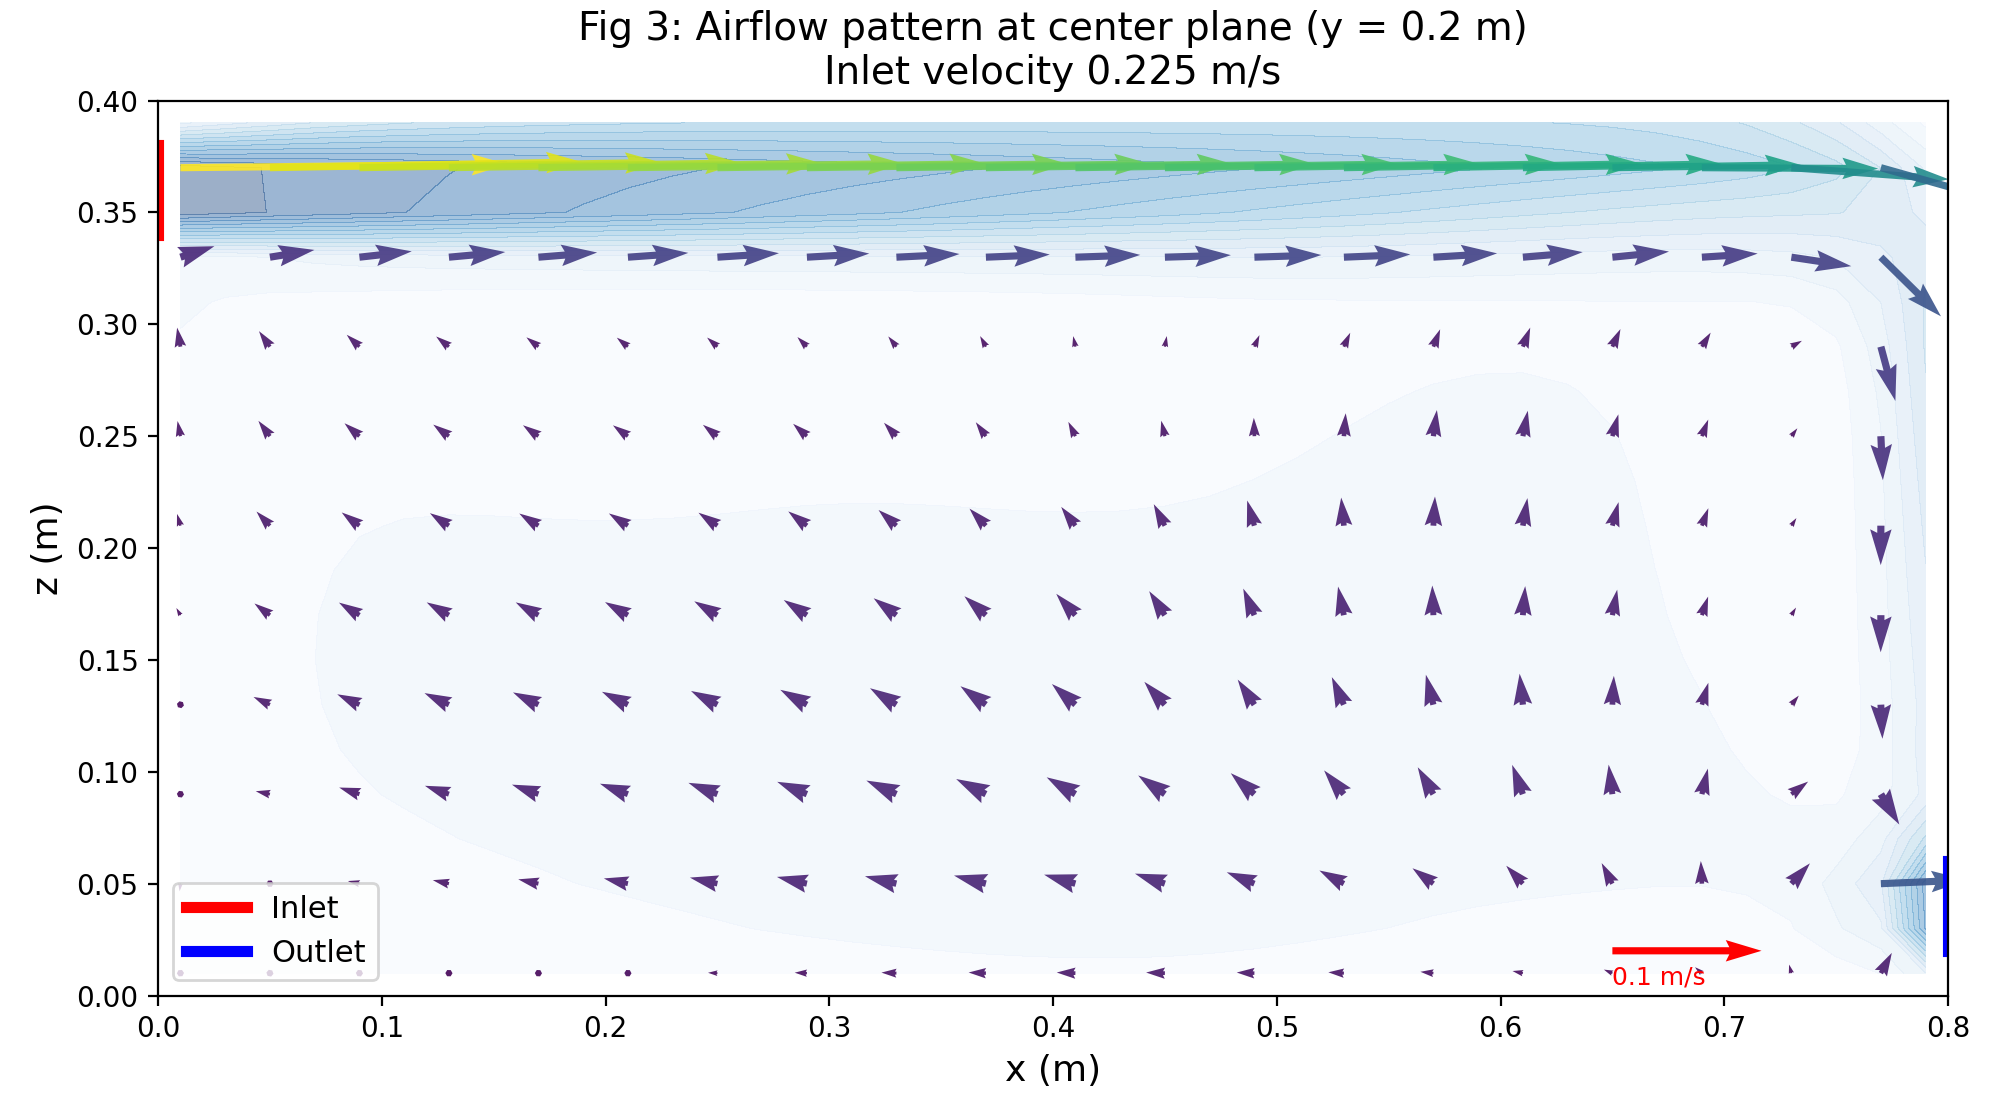
\includegraphics[width=0.85\textwidth]{figures/fig3_velocity_field.png}
\caption{Velocity field magnitude at the center plane ($y = 0.2\,$m) for Case~1 ($U = \SI{0.225}{\meter\per\second}$).}
\label{fig:velocity}
\end{figure}

Figure~\ref{fig:profiles} shows the x-direction velocity profiles at three streamwise locations ($x = 0.2, 0.4, 0.6\,$m) in the center plane. The jet peak near the ceiling ($z \approx 0.36\,$m) decays from $0.19\,$m/s at $x = 0.2\,$m to $0.14\,$m/s at $x = 0.6\,$m, while a weak return flow ($U_x \approx -0.02$ to $-0.04\,$m/s) is visible near the floor.

\begin{figure}[H]
\centering
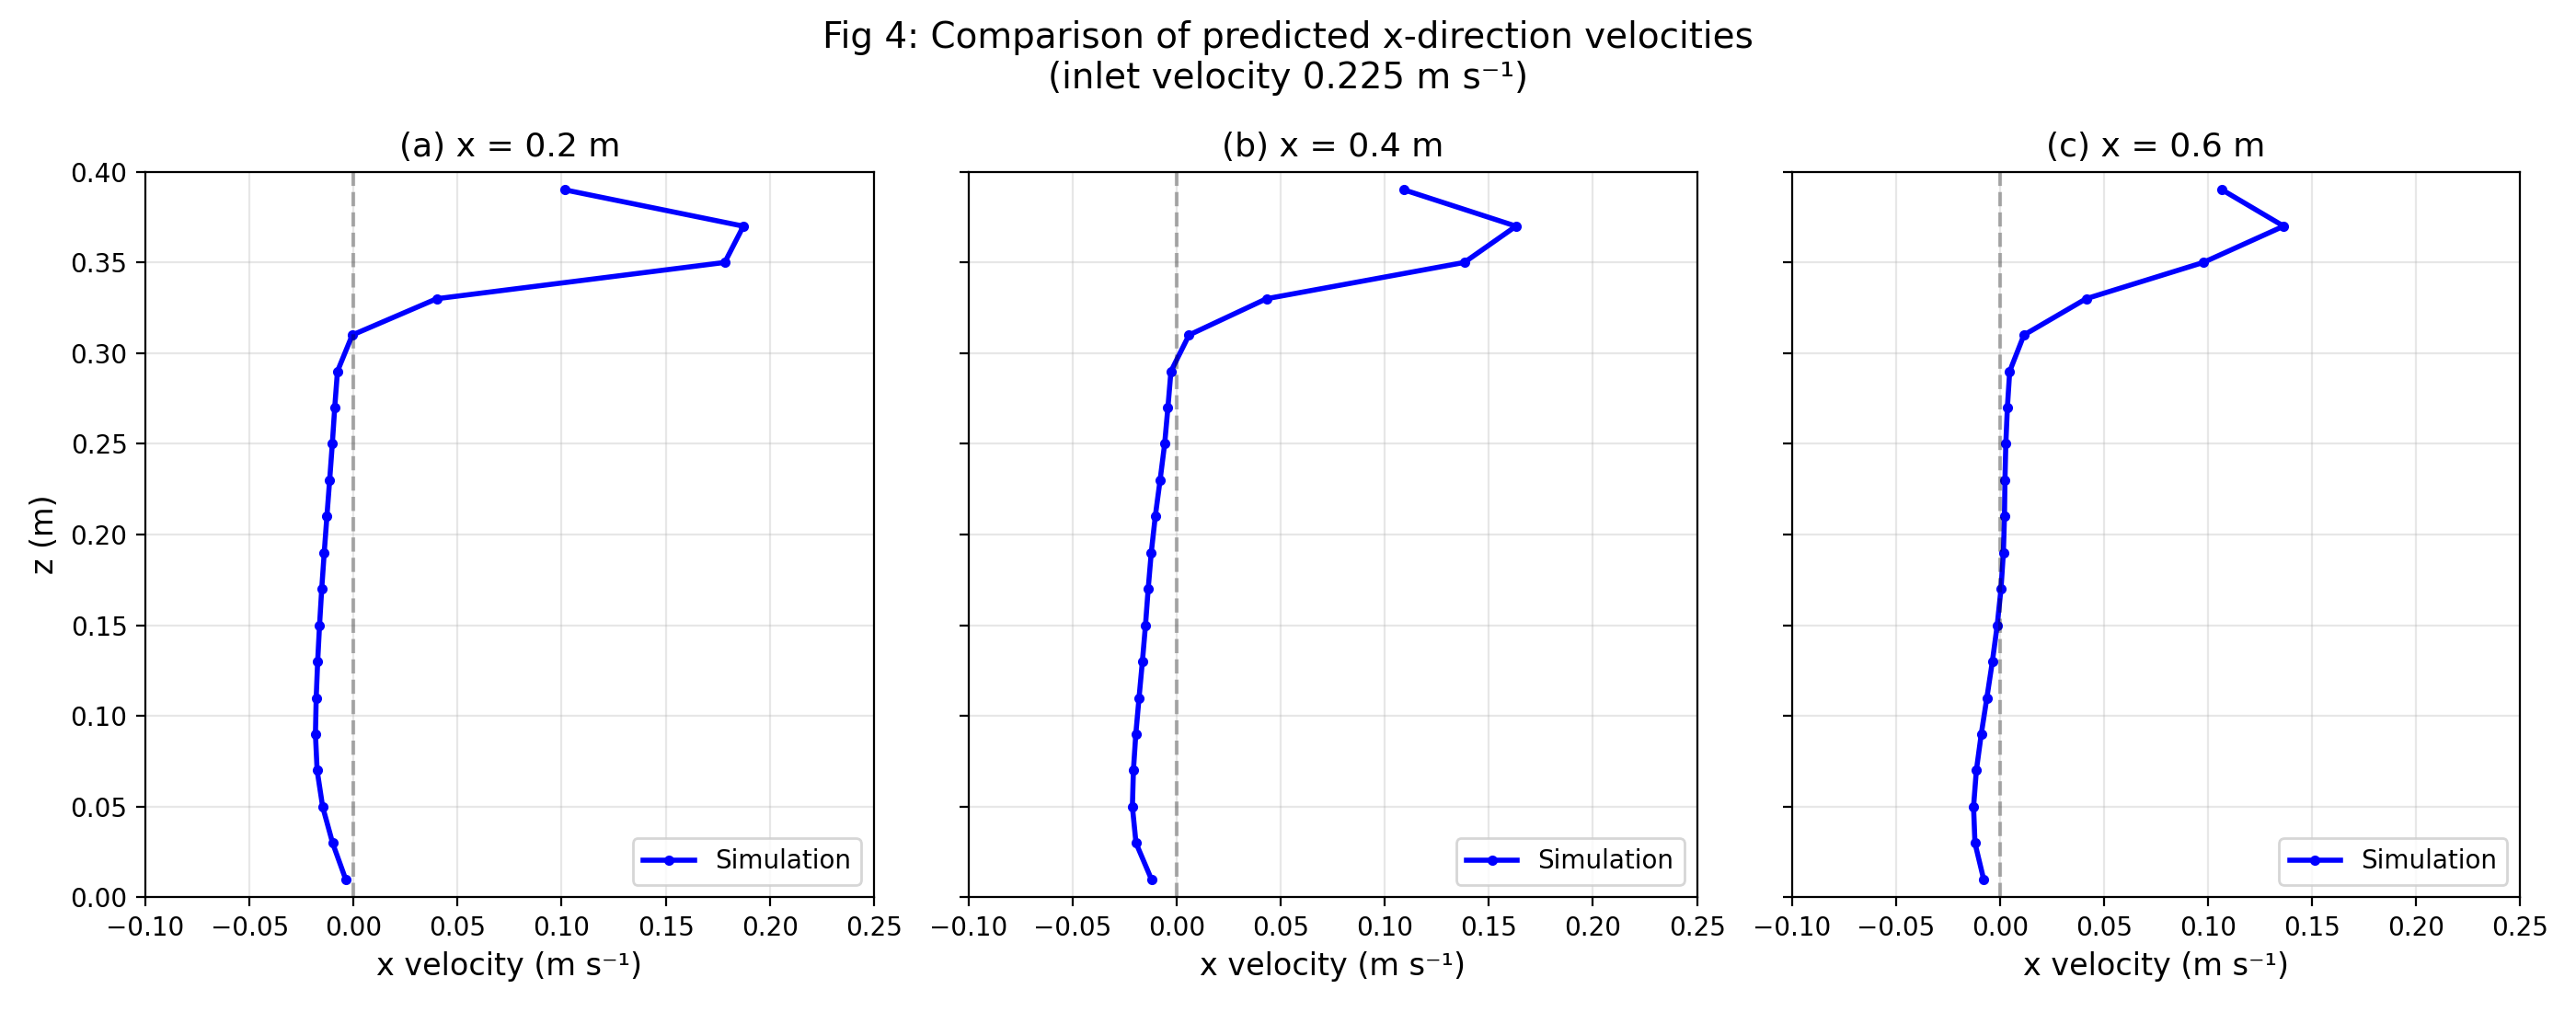
\includegraphics[width=0.95\textwidth]{figures/fig4_velocity_profiles.png}
\caption{Predicted x-direction velocity profiles at three streamwise locations in the center plane ($y = 0.2\,$m), Case~1.}
\label{fig:profiles}
\end{figure}

%----------------------------------------------------------------------------
\subsection{Concentration Evolution}
%----------------------------------------------------------------------------

Figure~\ref{fig:conc_evol} shows the normalized concentration field at the center plane at $t = 60, 180, 300, 1800\,$s for $1\,\mu$m (top row) and $10\,\mu$m (bottom row) particles. The $1\,\mu$m particles progressively fill the room toward a nearly uniform concentration by $t = 1800\,$s (CV~$= 4.5\%$). In contrast, the $10\,\mu$m particles exhibit strong vertical stratification due to gravitational settling, with concentration accumulating near the floor and depleting near the ceiling.

\begin{figure}[H]
\centering
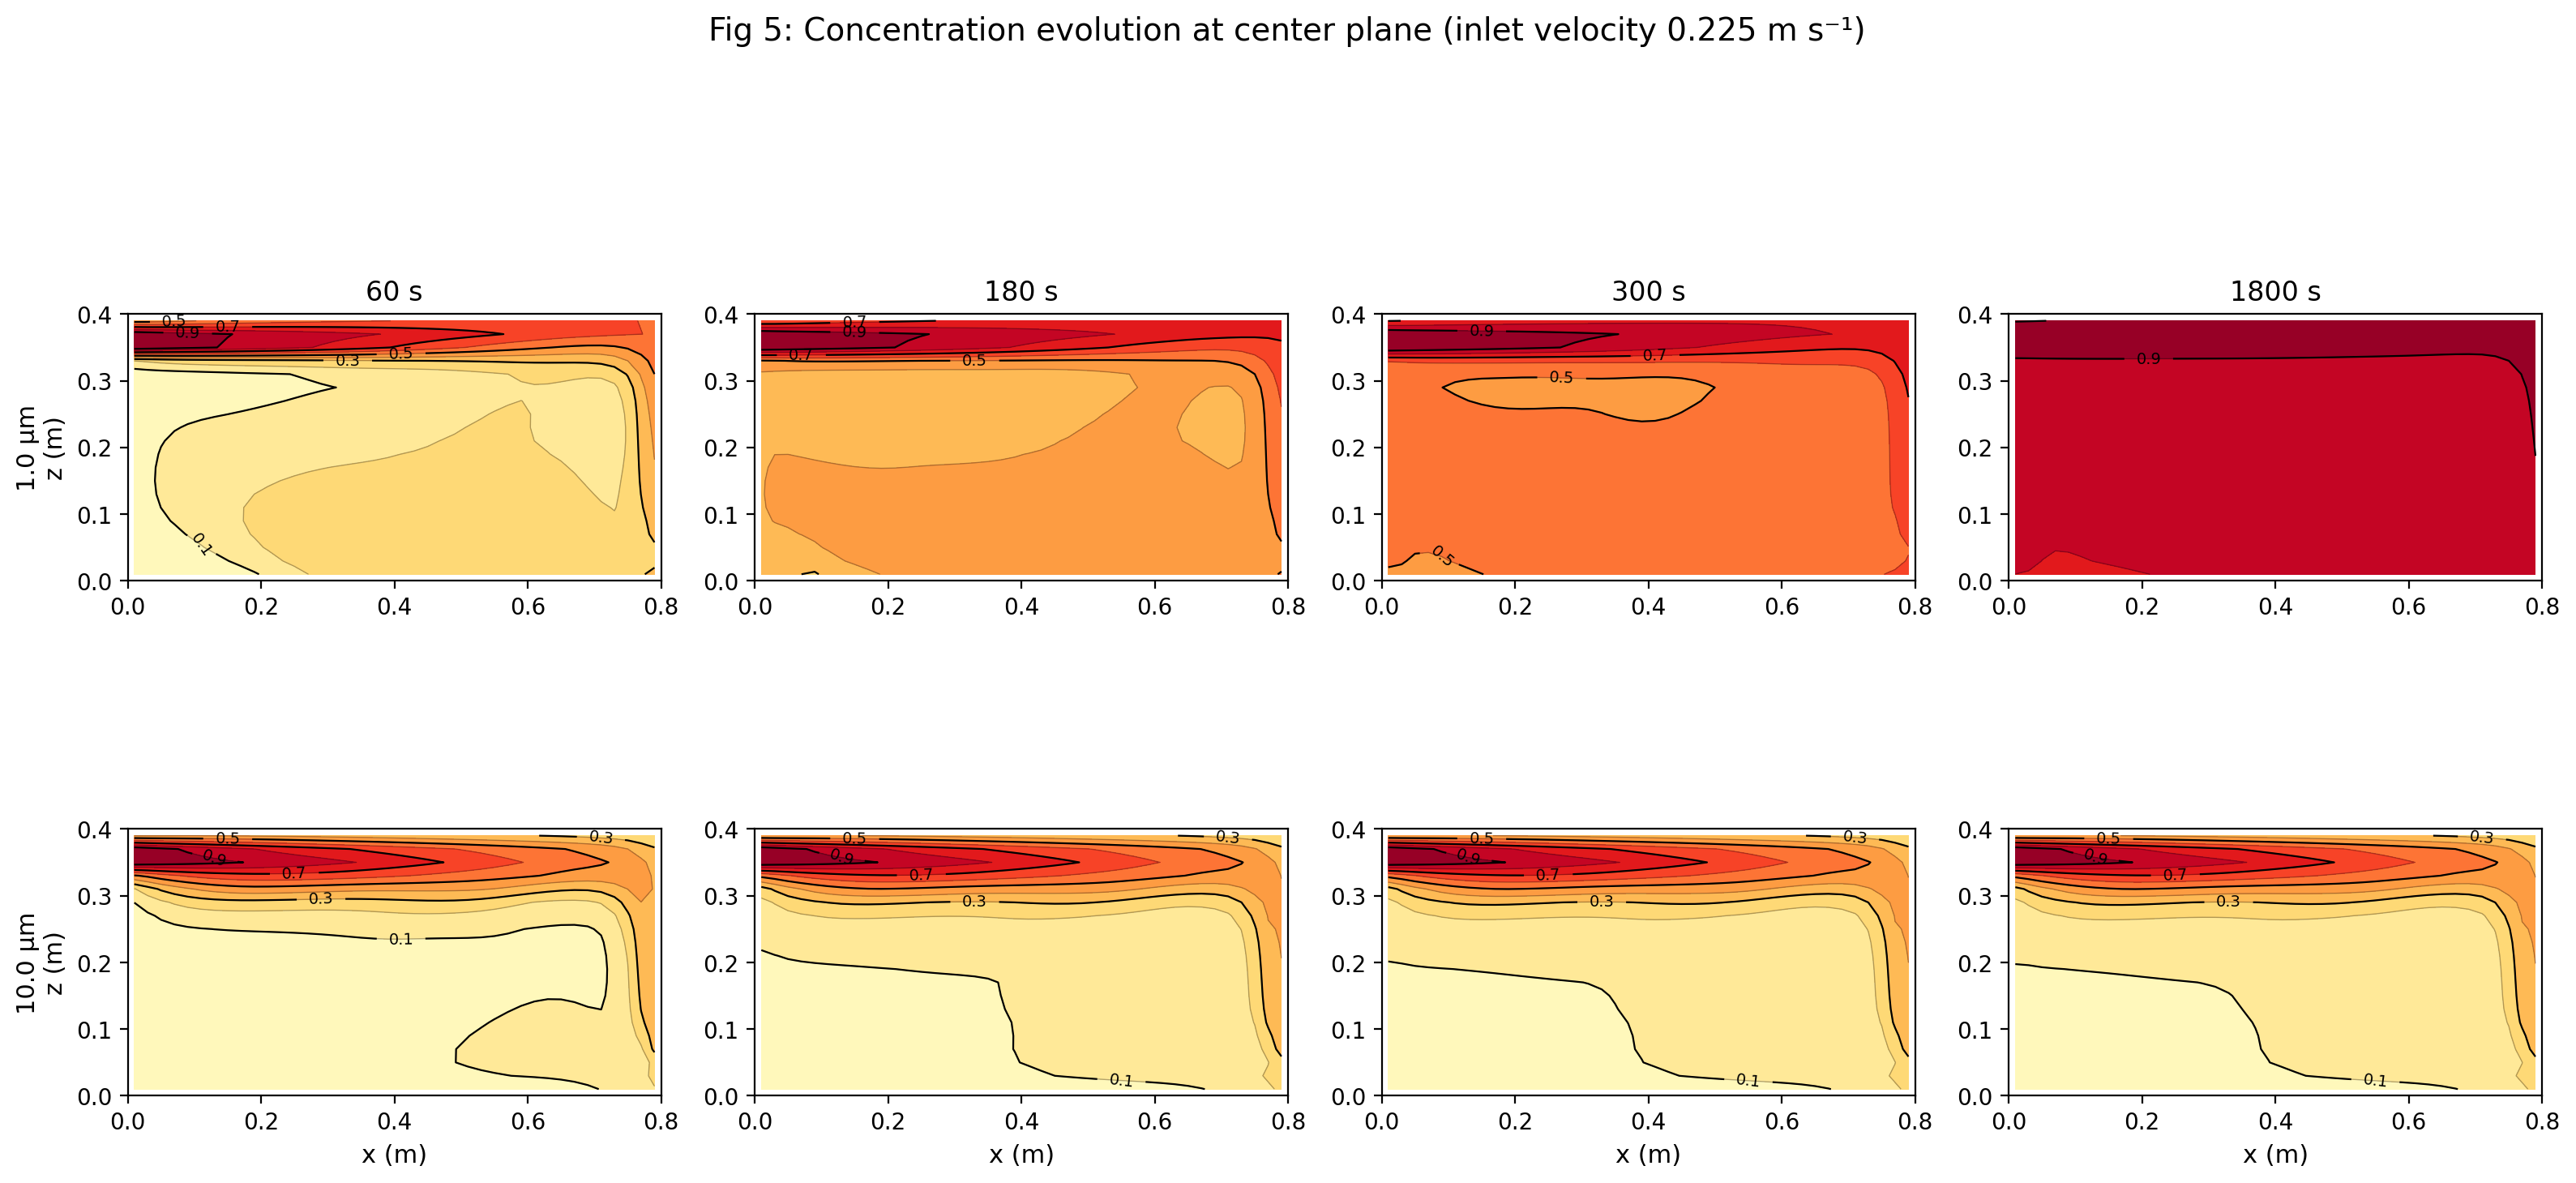
\includegraphics[width=0.95\textwidth]{figures/fig5_concentration_evolution.png}
\caption{Concentration evolution at the center plane for $1\,\mu$m (top) and $10\,\mu$m (bottom) particles at $t = 60, 180, 300, 1800\,$s. Case~1, $U = \SI{0.225}{\meter\per\second}$.}
\label{fig:conc_evol}
\end{figure}

%----------------------------------------------------------------------------
\subsection{Mixing Dynamics}
%----------------------------------------------------------------------------

Figure~\ref{fig:cv_time} shows the coefficient of variation (CV) versus time for selected particle sizes at both inlet velocities. Solid lines represent Case~1 ($U = 0.225\,$m/s), dashed lines Case~2 ($U = 0.45\,$m/s). Particles of $1\,\mu$m diameter cross the 10\% well-mixed threshold at $t \approx 540\,$s in Case~1 and $t \approx 180\,$s in Case~2, while $10\,\mu$m particles never reach the threshold in either case.

\begin{figure}[H]
\centering
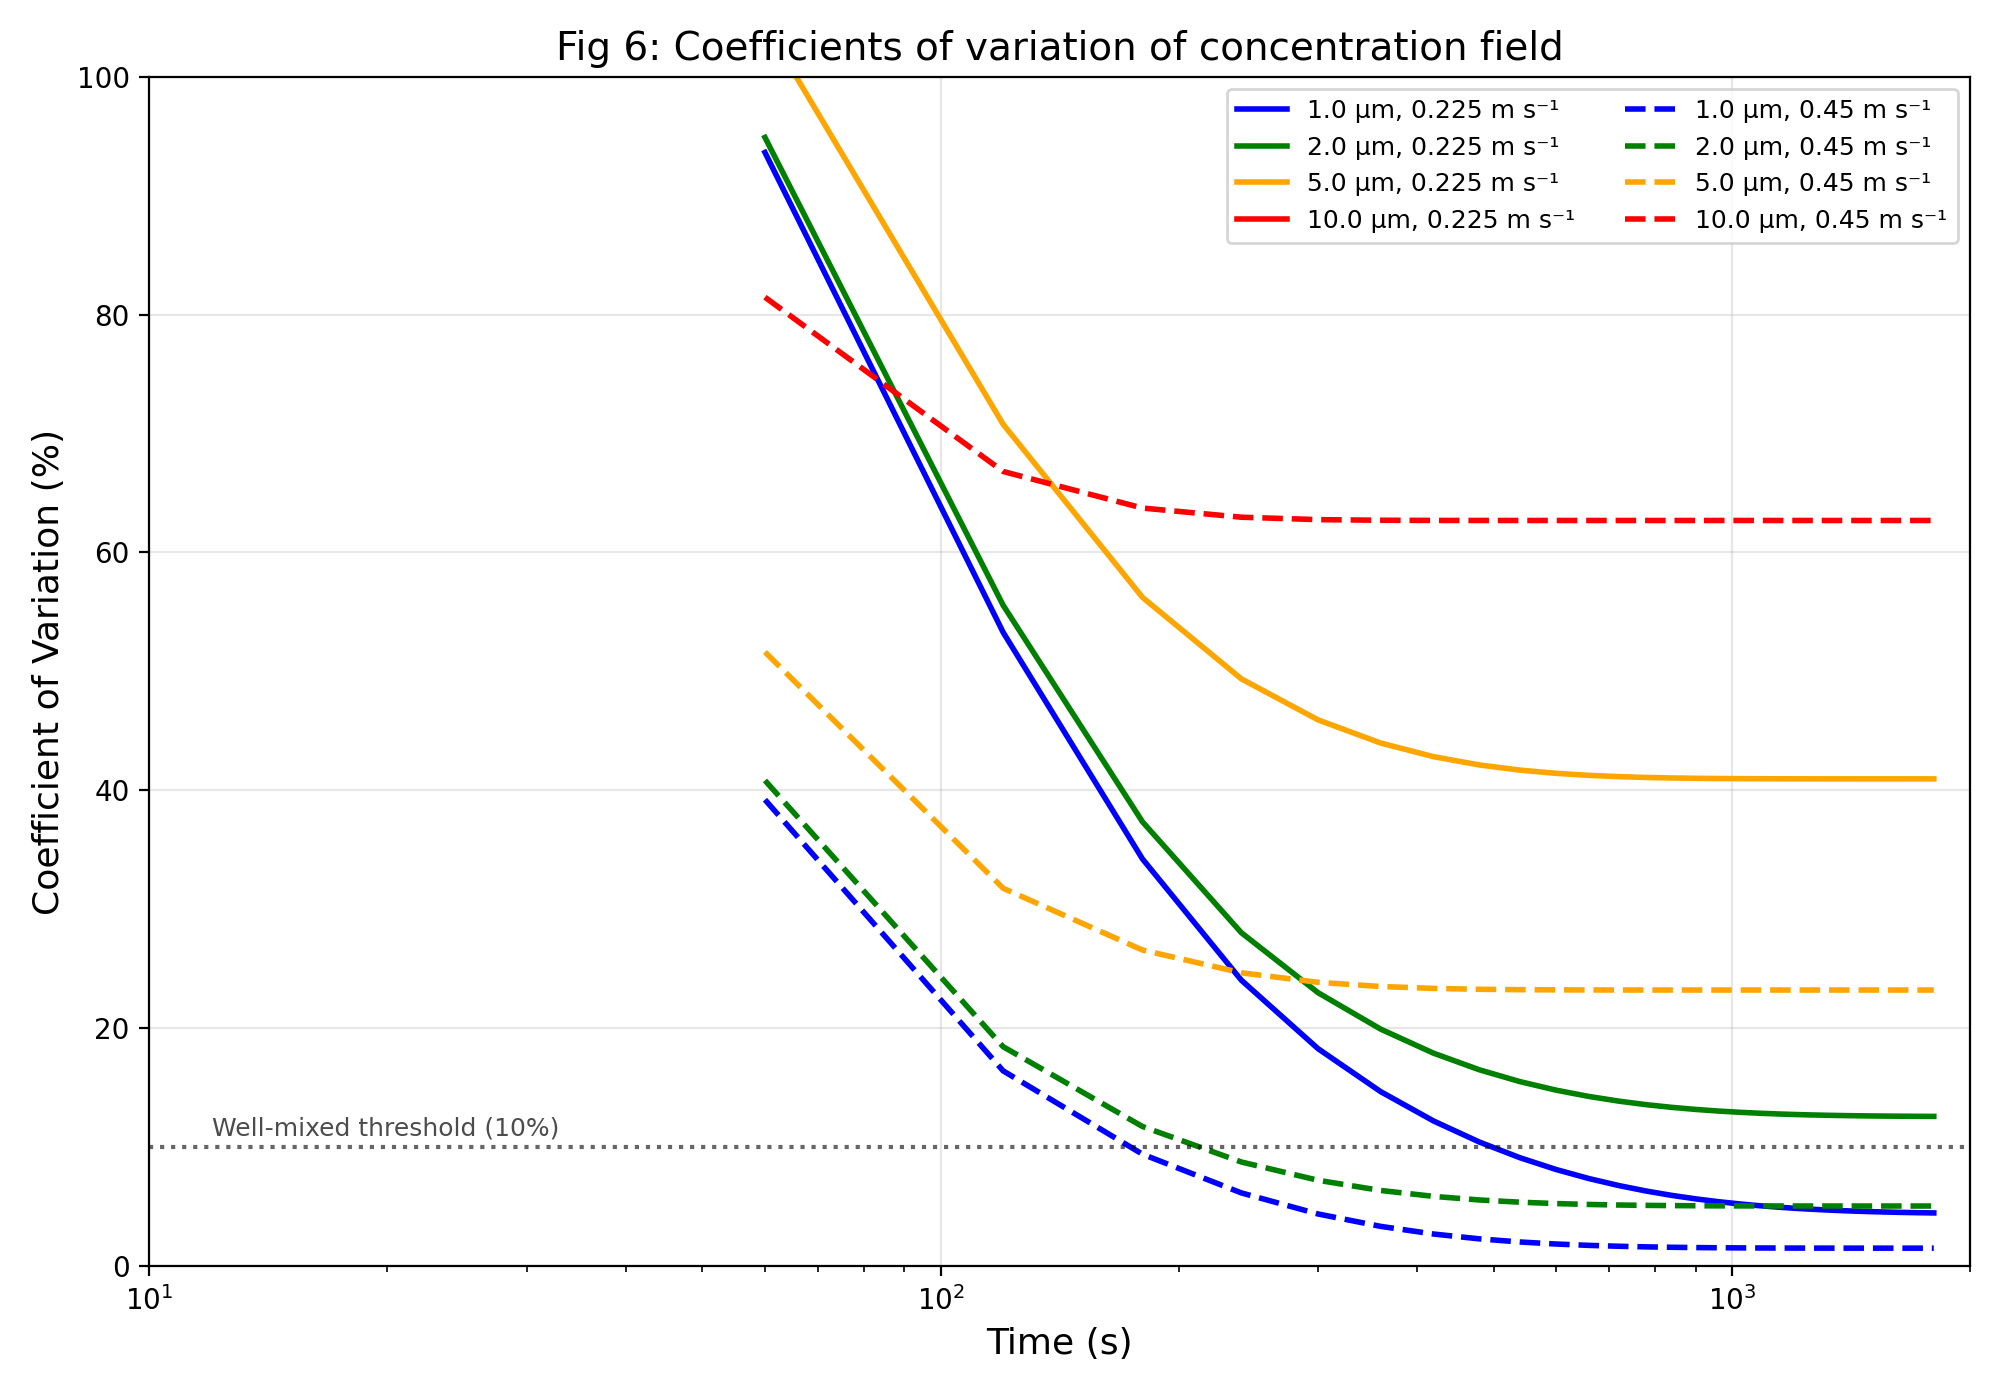
\includegraphics[width=0.85\textwidth]{figures/fig6_cv_timeseries.png}
\caption{Coefficient of variation versus time for selected particle sizes. Solid: Case~1 ($U = 0.225\,$m/s), dashed: Case~2 ($U = 0.45\,$m/s). Dotted line marks the 10\% well-mixed threshold.}
\label{fig:cv_time}
\end{figure}

Figure~\ref{fig:conc_profiles} shows vertical concentration profiles for $10\,\mu$m particles at $t = 1800\,$s at three streamwise locations. The strong vertical gradient confirms that gravitational settling dominates the particle distribution for coarse particles, producing concentrations $2$--$5\times$ higher near the floor than near the ceiling.

\begin{figure}[H]
\centering
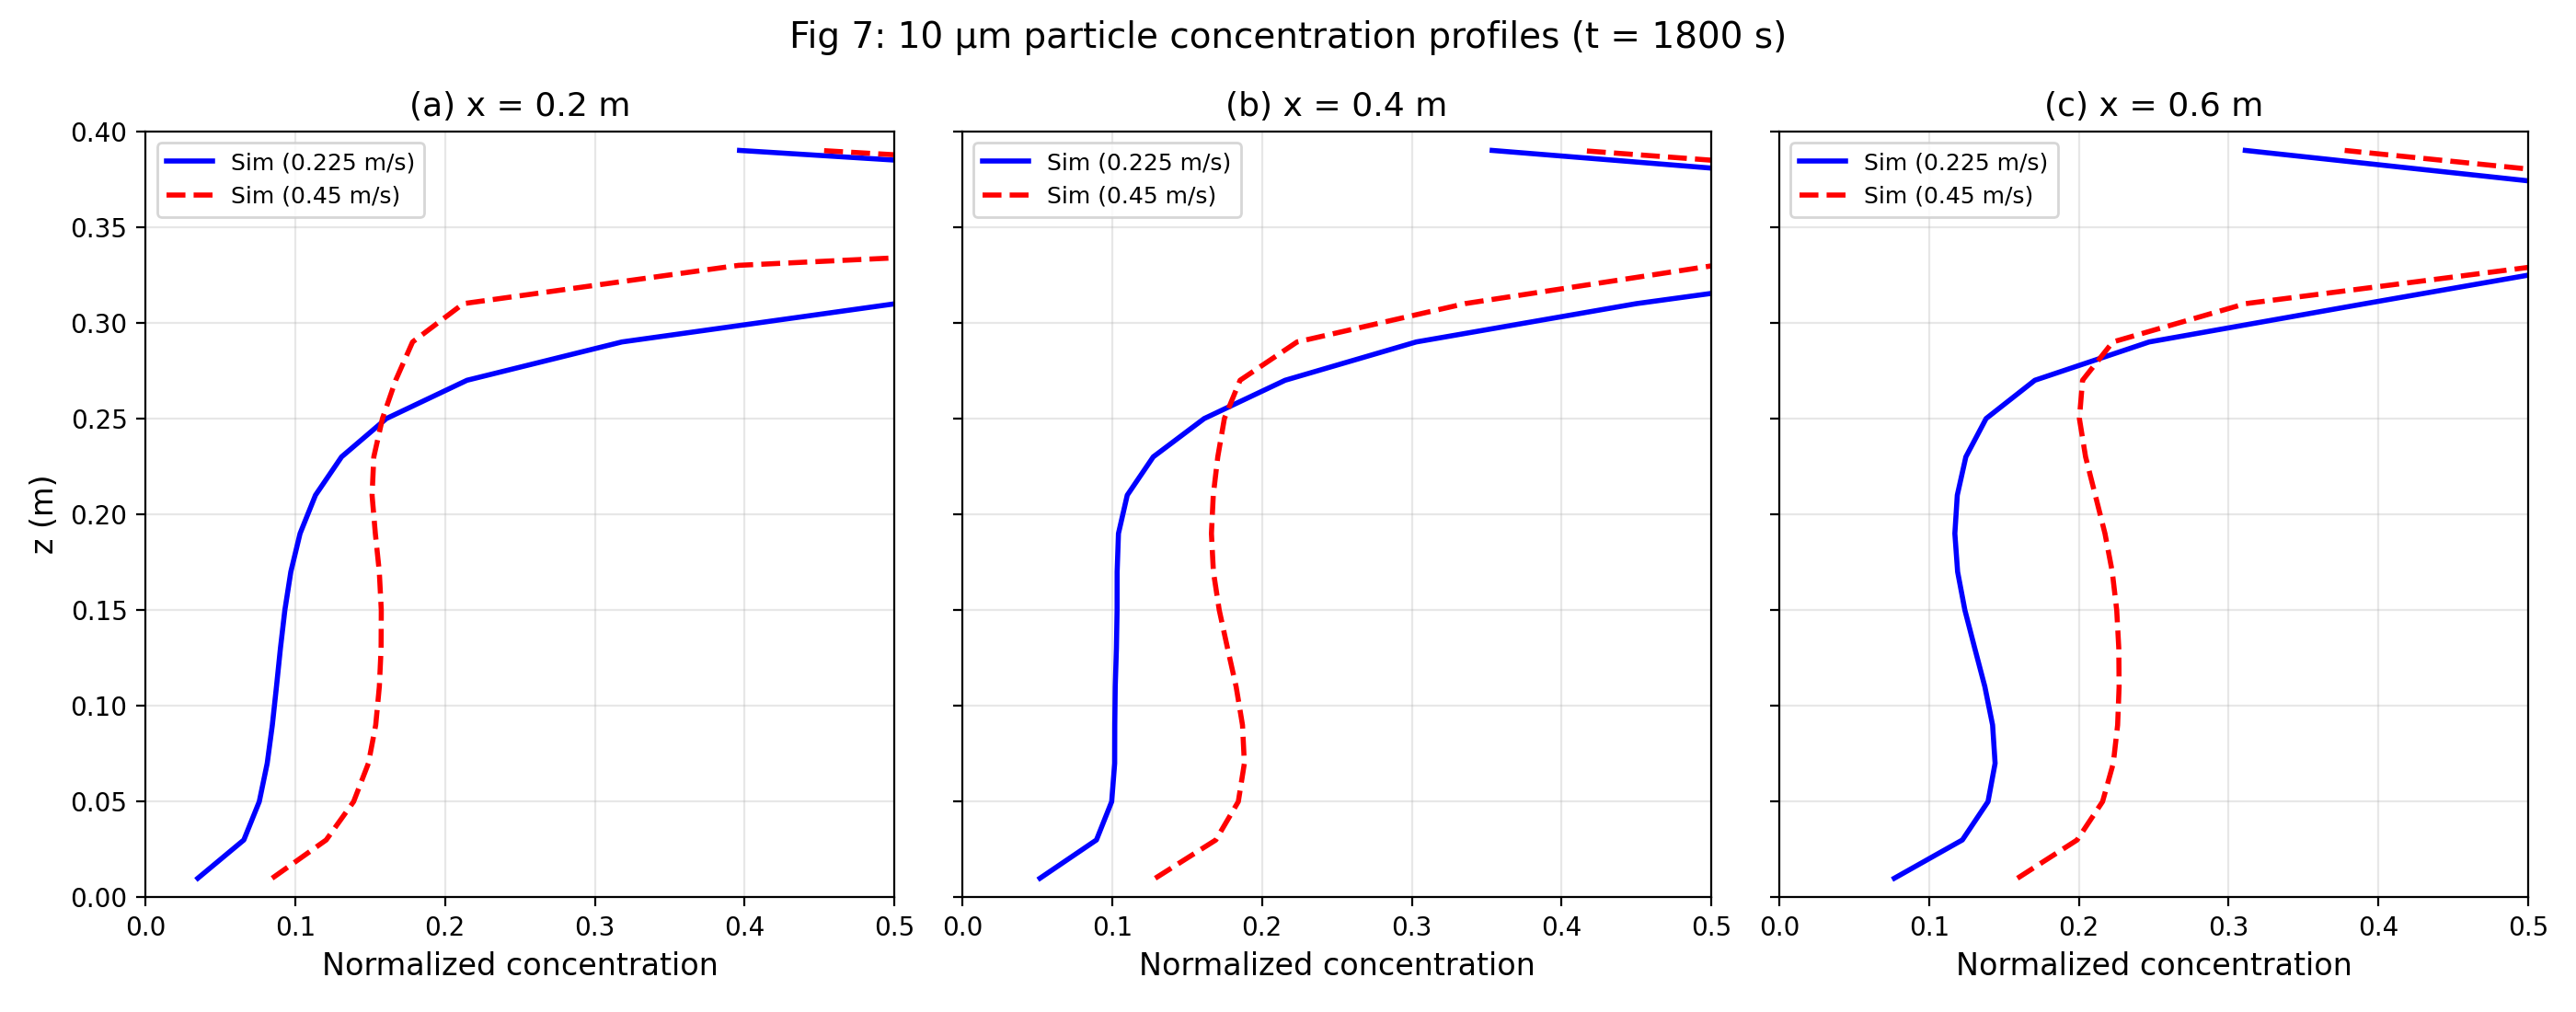
\includegraphics[width=0.95\textwidth]{figures/fig7_concentration_profiles.png}
\caption{Vertical concentration profiles of $10\,\mu$m particles at $t = 1800\,$s, at $x = 0.2, 0.4, 0.6\,$m in the center plane.}
\label{fig:conc_profiles}
\end{figure}

%----------------------------------------------------------------------------
\subsection{Particle Transport Results}
%----------------------------------------------------------------------------

Table~\ref{tab:results} summarizes the mixing time, final coefficient of variation, and mean dimensionless concentration for all particle sizes and both cases.

\begin{table}[H]
\centering
\caption{Summary of particle transport results at $t = 1800\,$s. Mixing time is the first time at which CV~$< 10\%$.}
\label{tab:results}
\small
\begin{tabular}{cc|ccc|ccc}
\toprule
&& \multicolumn{3}{c|}{\textbf{Case 1: $U = \SI{0.225}{\meter\per\second}$}} & \multicolumn{3}{c}{\textbf{Case 2: $U = \SI{0.45}{\meter\per\second}$}} \\
\cmidrule(lr){3-5}\cmidrule(lr){6-8}
$d_p$ ($\mu$m) & $v_s$ (m/s) & $t_\text{mix}$ (s) & CV & $\langle C^+ \rangle$ & $t_\text{mix}$ (s) & CV & $\langle C^+ \rangle$ \\
\midrule
0.01  & $1.87\times10^{-07}$ & 480 & 0.018 & 0.933 & 180 & 0.012 & 0.942 \\
0.05  & $9.86\times10^{-07}$ & 420 & 0.004 & 0.982 & 180 & 0.002 & 0.992 \\
0.10  & $2.11\times10^{-06}$ & 420 & 0.004 & 0.982 & 180 & 0.001 & 0.995 \\
0.50  & $1.78\times10^{-05}$ & 480 & 0.016 & 0.937 & 180 & 0.005 & 0.974 \\
1.00  & $5.62\times10^{-05}$ & 540 & 0.045 & 0.842 & 180 & 0.015 & 0.923 \\
2.00  & $1.97\times10^{-04}$ & --- & 0.126 & 0.631 & 240 & 0.051 & 0.778 \\
3.00  & $4.21\times10^{-04}$ & --- & 0.217 & 0.469 & --- & 0.102 & 0.627 \\
5.00  & $1.12\times10^{-03}$ & --- & 0.410 & 0.280 & --- & 0.232 & 0.402 \\
7.00  & $2.16\times10^{-03}$ & --- & 0.646 & 0.182 & --- & 0.384 & 0.273 \\
10.00 & $4.36\times10^{-03}$ & --- & 1.003 & 0.121 & --- & 0.627 & 0.174 \\
\bottomrule
\end{tabular}
\end{table}

%----------------------------------------------------------------------------
\subsection{Key Observations}
%----------------------------------------------------------------------------

\textbf{Mixing time decreases with doubled ventilation:} For the smallest particles ($d_p \le \SI{1}{\micro\meter}$), the mixing time halves from approximately $420$--$540\,$s to $180\,$s when the ventilation rate doubles. This directly reflects the enhanced turbulent mixing at higher flow rates.

\textbf{Deposition dominates for large particles:} Particles with $d_p \ge \SI{2}{\micro\meter}$ fail to reach CV~$< 10\%$ within 30 minutes in both cases. The final mean concentration $\langle C^+ \rangle$ drops below $0.65$ for $d_p = \SI{2}{\micro\meter}$ and below $0.13$ for $d_p = \SI{10}{\micro\meter}$, indicating that strong gravitational settling and wall deposition remove most particles from the air before uniform mixing can occur.

\textbf{Optimal mixing at intermediate sizes:} The $0.05$--$\SI{0.1}{\micro\meter}$ range shows the fastest convergence to uniform concentration (CV~$< 0.005$ and $\langle C^+ \rangle \approx 0.98$). These particles are small enough to have negligible settling but large enough that Brownian diffusion is weak, so they closely follow the airflow streamlines.

\textbf{Size-dependent behavior:} Figure~\ref{fig:cv} shows the coefficient of variation versus particle diameter. A clear transition from diffusion-dominated (small $d_p$, rapid mixing) to settling-dominated (large $d_p$, incomplete mixing) is visible, with the crossover occurring around $d_p \approx \SI{1}{\micro\meter}$.

\begin{figure}[H]
\centering
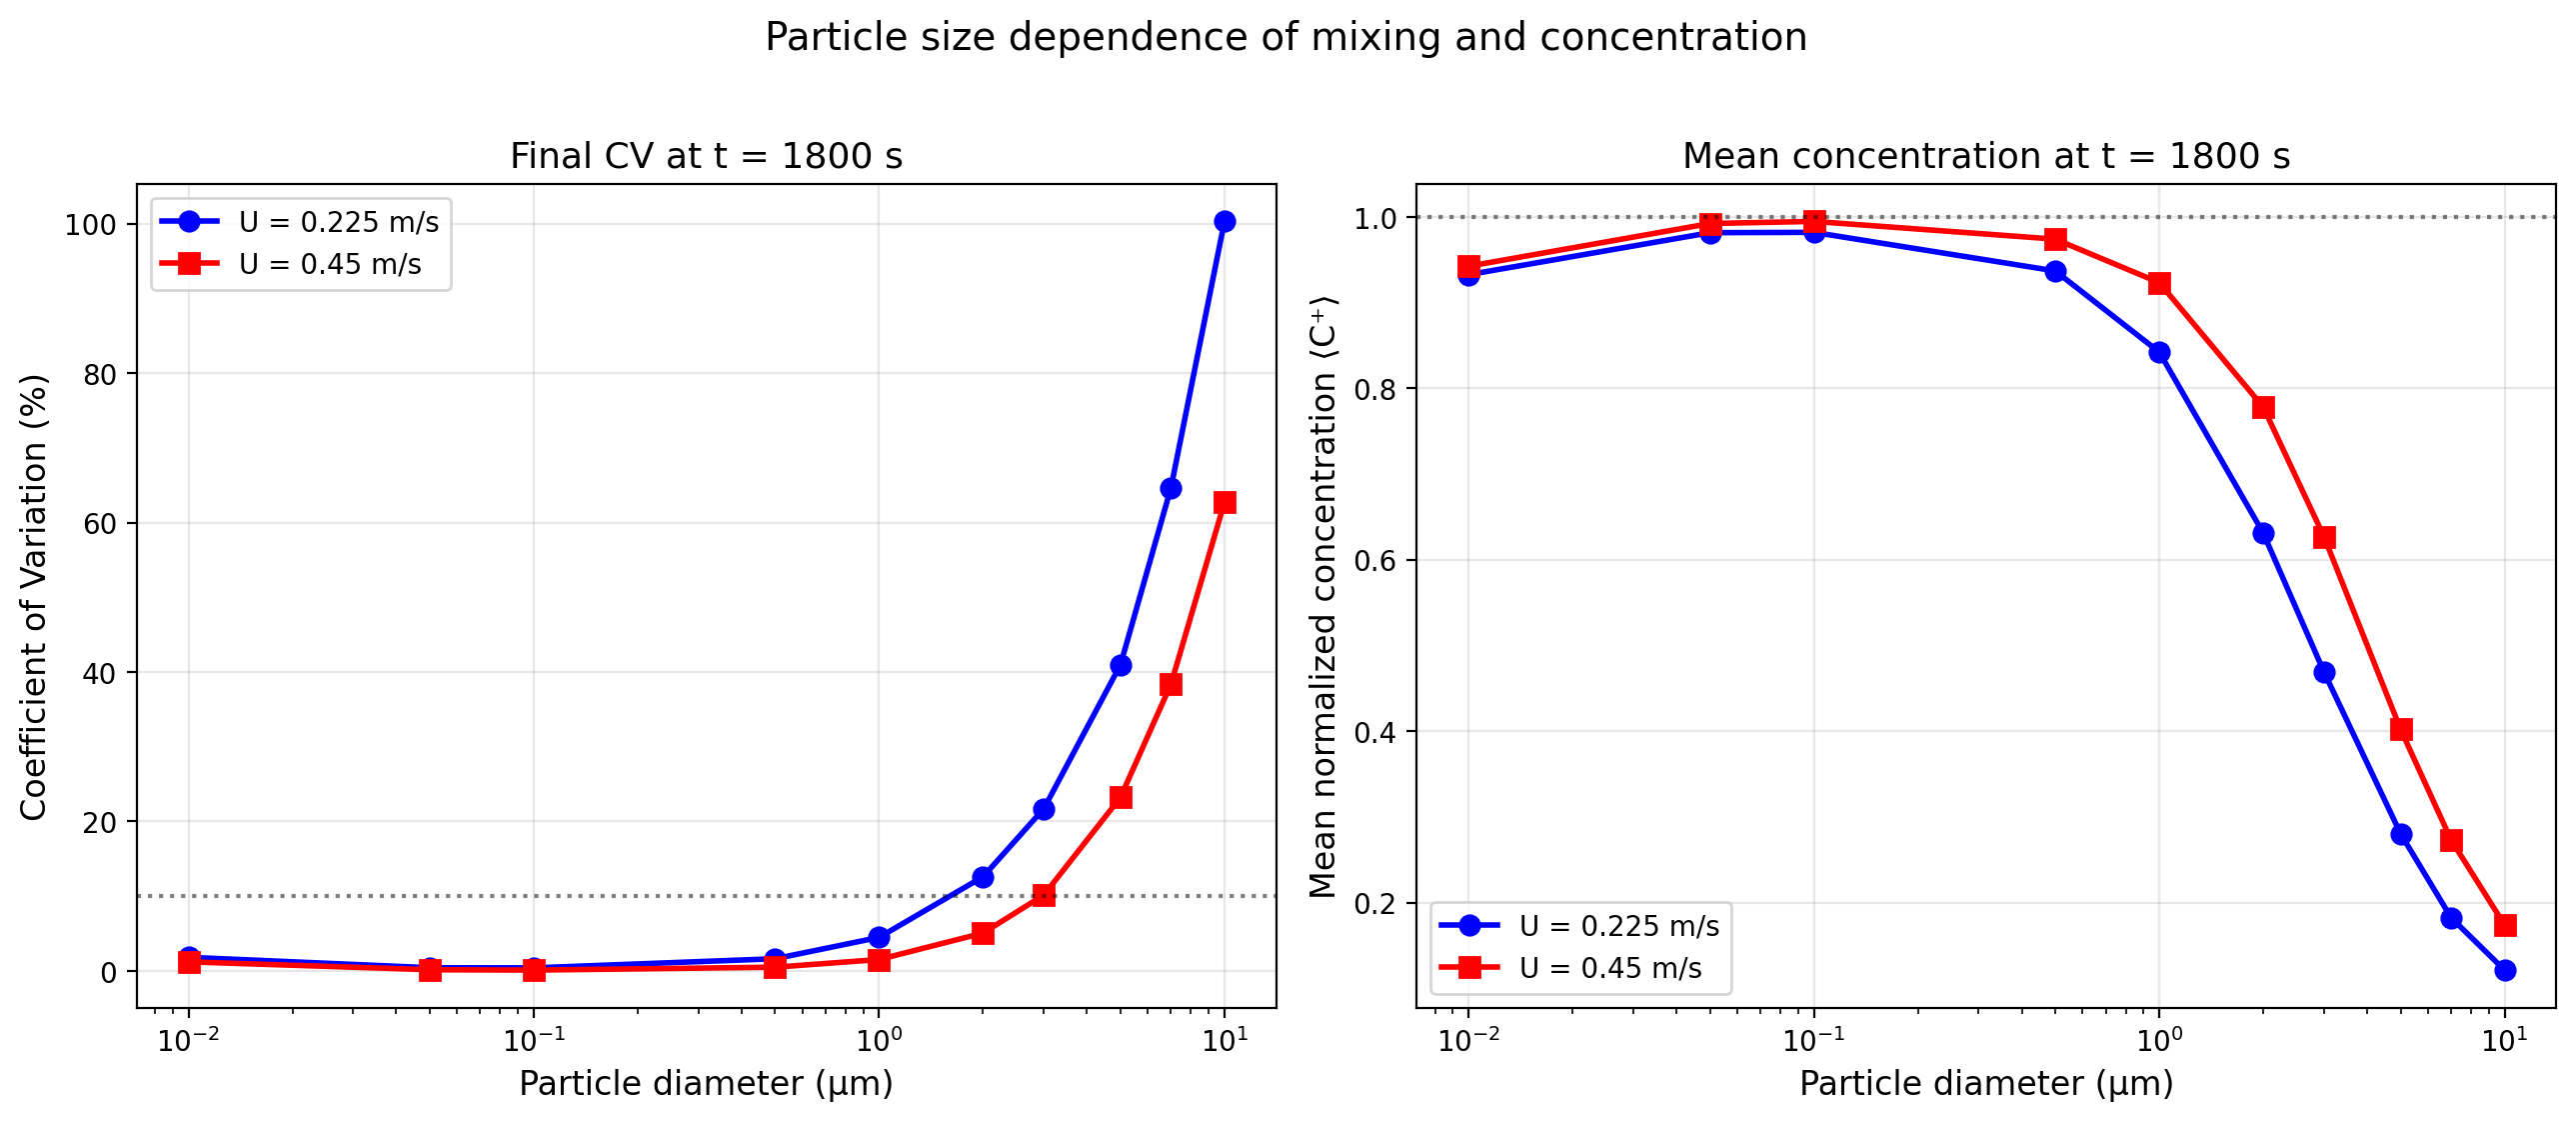
\includegraphics[width=0.85\textwidth]{figures/cv_vs_diameter.png}
\caption{Final coefficient of variation (left) and mean normalized concentration (right) versus particle diameter for both cases at $t = 1800\,$s.}
\label{fig:cv}
\end{figure}

Figure~\ref{fig:summary} presents a color-coded summary of all results for Case~1, with green indicating well-mixed conditions (CV~$< 10\%$), yellow indicating borderline mixing, and red indicating non-uniform distribution.

\begin{figure}[H]
\centering
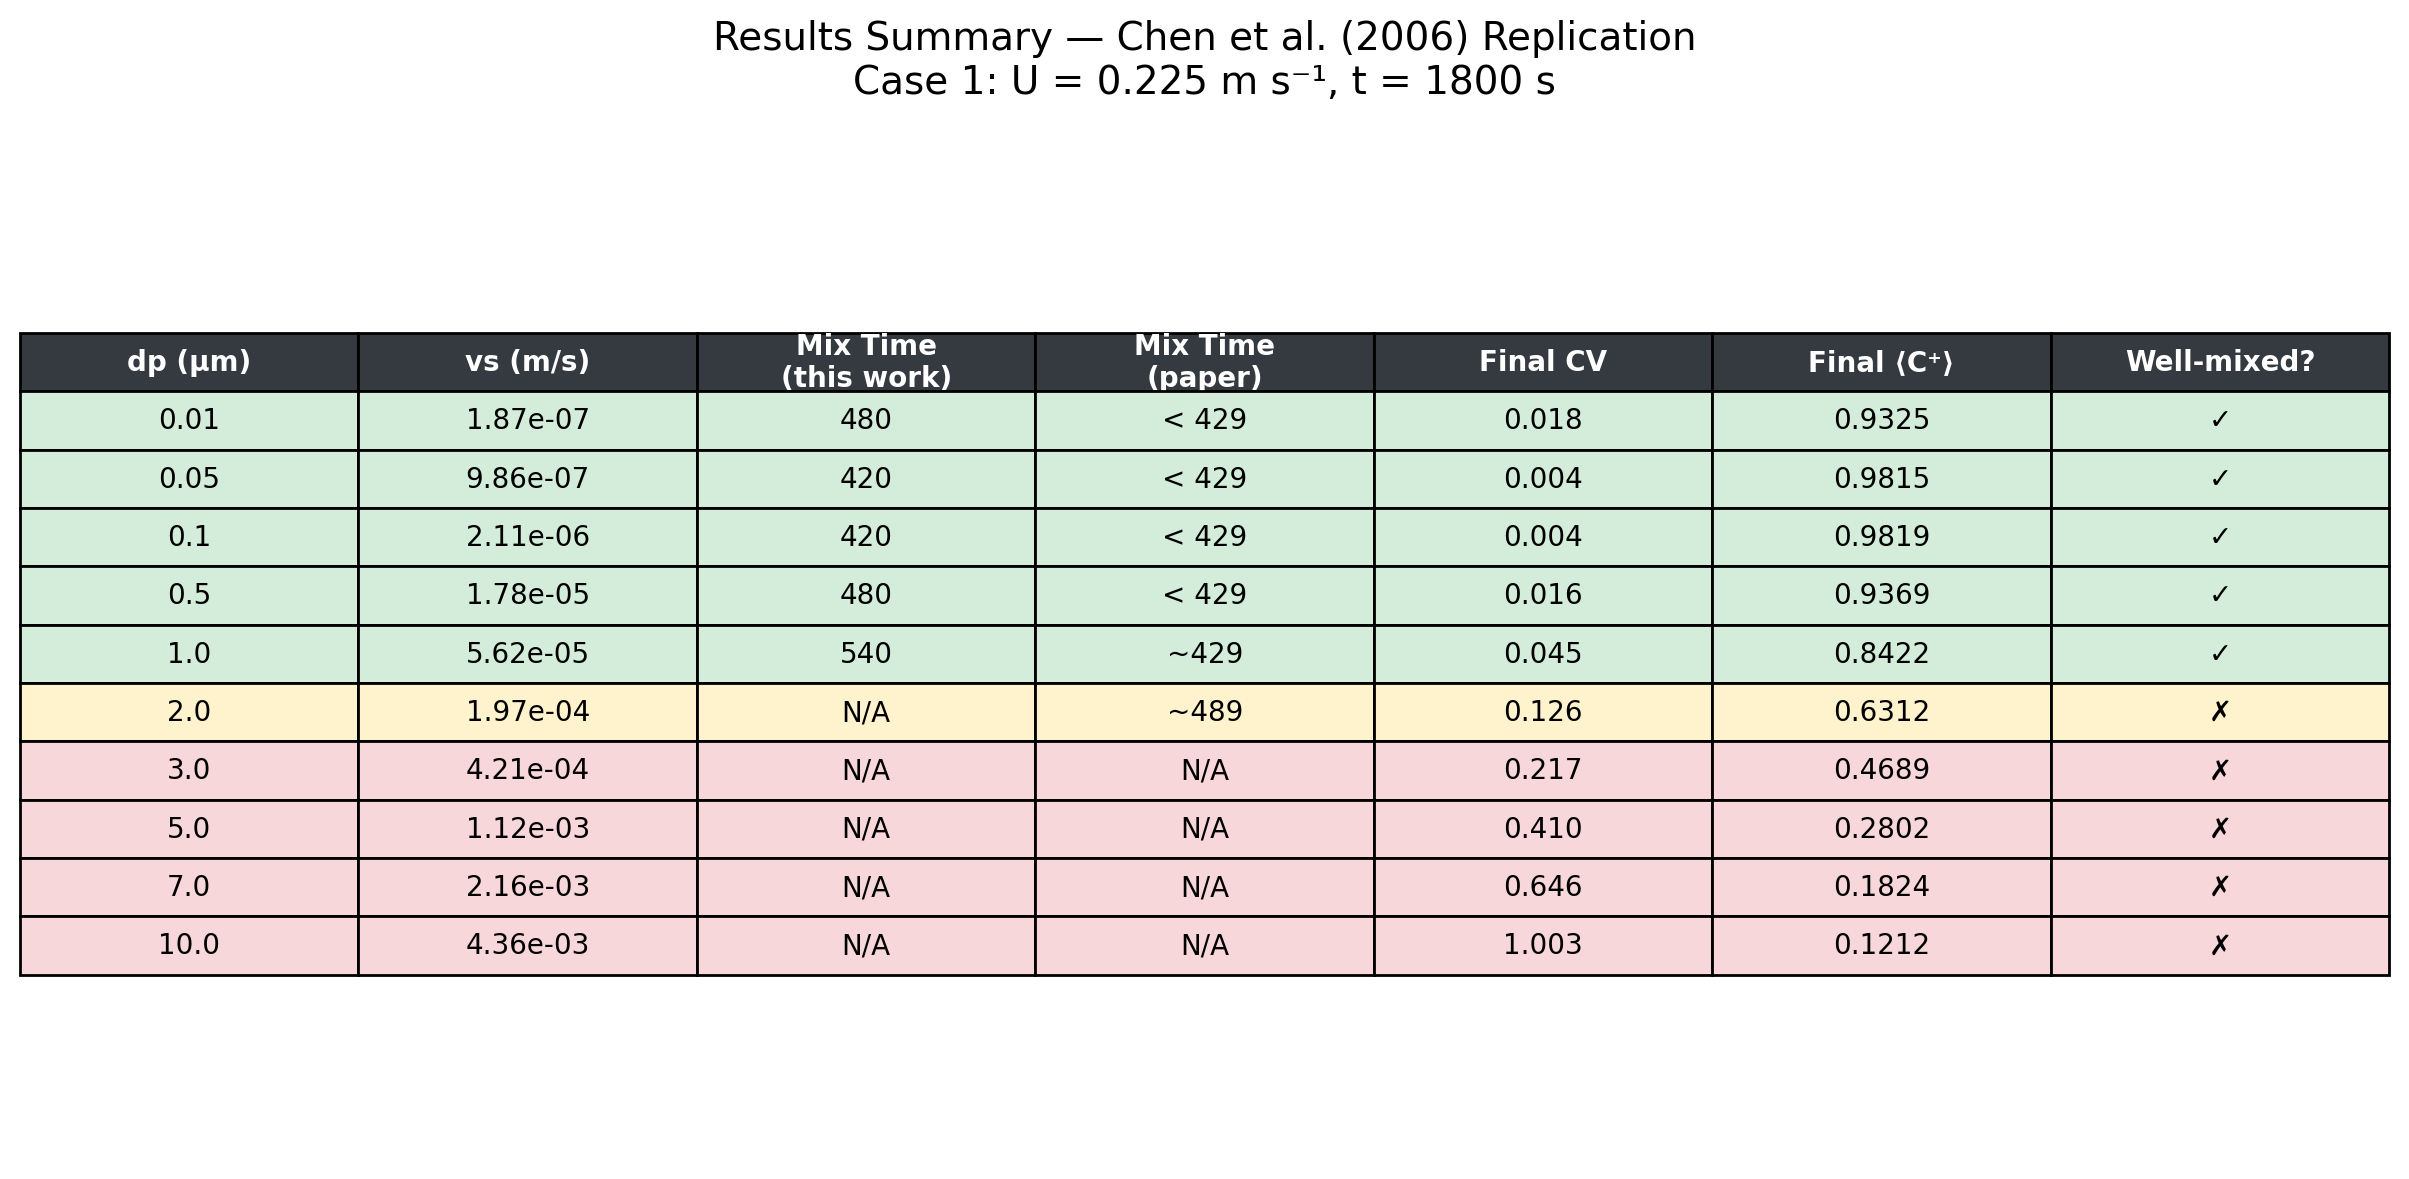
\includegraphics[width=0.85\textwidth]{figures/summary_table.png}
\caption{Color-coded summary of particle transport results for Case~1. Green: well-mixed (CV~$< 10\%$), yellow: borderline, red: non-uniform.}
\label{fig:summary}
\end{figure}

%============================================================================
\section{HPC Exercise: Running on ALCF Systems}
%============================================================================

This section provides a hands-on exercise for deploying the same OpenFOAM drift-flux airflow case on three high-performance computing platforms at the Argonne Leadership Computing Facility (ALCF). The particle transport step (Python solver) need not be run on the HPC systems---it can be executed locally after downloading the airflow fields---but the steady-state OpenFOAM simulation itself serves as an excellent first CFD benchmark on each architecture.

\begin{table}[H]
\centering
\caption{ALCF platform specifications relevant to this exercise.}
\begin{tabular}{lccc}
\toprule
\textbf{Platform} & \textbf{GPUs/Node} & \textbf{CPU} & \textbf{Scheduler} \\
\midrule
Aurora & 6$\times$ Intel Max 1550 & Xeon CPU Max & PBS \\
Polaris & 4$\times$ NVIDIA A100-SXM4-40GB & AMD EPYC Milan & PBS \\
chiatta00 (JLSE) & 8$\times$ Intel Data Center Max & Xeon & None (interactive) \\
\bottomrule
\end{tabular}
\end{table}

%----------------------------------------------------------------------------
\subsection{Preparing the Case (Common Steps)}
%----------------------------------------------------------------------------

Before submitting to any platform, prepare a tarball of the OpenFOAM case from your local workstation:

\begin{lstlisting}[language=bash]
$ cd ~/Dropbox/REPLICATE-PROJECT/drift-flux-indoor-particles/code
$ tar czf openfoam-case.tgz openfoam/
\end{lstlisting}

This archive contains the complete case directory (\texttt{0/}, \texttt{constant/}, \texttt{system/}) ready for deployment.

%----------------------------------------------------------------------------
\subsection{Case A: Aurora (Intel GPU Cluster)}
%----------------------------------------------------------------------------

Aurora is ALCF's exascale system with Intel Max 1550 GPUs. For this exercise we run OpenFOAM on CPU cores; GPU-accelerated solvers (via OGL/Ginkgo) are a separate advanced topic.

\textbf{OpenFOAM installation:} OpenFOAM v2412 is already compiled at:\
\texttt{\textasciitilde/software/cfd-comparison/OpenFOAM-v2412/}

\textbf{Job script} (\texttt{aurora\_job.sh}):

\begin{lstlisting}[language=bash]
#!/bin/bash
#PBS -N drift_flux_aurora
#PBS -A datascience
#PBS -q workq
#PBS -l select=1
#PBS -l walltime=00:30:00
#PBS -j oe

export source ~/software/cfd-comparison/OpenFOAM-v2412/etc/bashrc

echo "=== Drift-Flux on Aurora ==="
echo "Working directory: $(pwd)"
echo "Hostname: $(hostname)"

# Generate mesh
echo "--- blockMesh ---"
blockMesh > log.blockMesh 2>&1

# Check mesh
echo "--- checkMesh ---"
checkMesh > log.checkMesh 2>&1

# Run steady-state solver
echo "--- simpleFoam ---"
simpleFoam > log.simpleFoam 2>&1

echo "=== Complete ==="
\end{lstlisting}

\textbf{Instructions to run:}
\begin{lstlisting}[language=bash, basicstyle=\ttfamily\small]
# 1. Copy case to Aurora (run from local workstation)
$ scp openfoam-case.tgz <username>@aurora.alcf.anl.gov:~/

# 2. Log in to Aurora
$ ssh <username>@aurora.alcf.anl.gov

# 3. Unpack and prepare
$ tar xzf openfoam-case.tgz
$ mv openfoam drift_flux_aurora
$ cd drift_flux_aurora

# 4. Submit job
$ qsub ../aurora_job.sh

# 5. Monitor
$ qstat -u $USER
\end{lstlisting}

\textbf{Expected runtime:} For 16,000 cells, \texttt{simpleFoam} completes in approximately $120$--$180$ seconds on Aurora CPU cores. The dominant cost is the pressure Poisson solve with GAMG preconditioning.

\textbf{Extracting results:}
\begin{lstlisting}[language=bash]
# After job completion, extract the final time directory
$ tar czf results_aurora.tgz 5000/ log.*
$ scp results_aurora.tgz <user>@<local_host>:~/Downloads/
\end{lstlisting}

%----------------------------------------------------------------------------
\subsection{Case B: Polaris (NVIDIA A100 Cluster)}
%----------------------------------------------------------------------------

Polaris features NVIDIA A100-SXM4-40GB GPUs on AMD EPYC Milan CPU nodes. OpenFOAM runs on CPU cores here as well; the A100s are not engaged for this serial steady-state solve.

\textbf{Checking for OpenFOAM:}
\begin{lstlisting}[language=bash]
$ module avail openfoam
\end{lstlisting}
If no module is available, you may build OpenFOAM from source or transfer the Aurora installation if compatible (both use Linux x86\_64; however, MPI libraries may differ).

\textbf{Job script} (\texttt{polaris\_job.sh}):

\begin{lstlisting}[language=bash]
#!/bin/bash
#PBS -N drift_flux_polaris
#PBS -A datascience
#PBS -q debug          # Use 'debug' for quick test; 'preemptable' for longer
#PBS -l select=1:ncpus=32:ngpus=4
#PBS -l walltime=00:30:00
#PBS -j oe

module load openfoam/...  # Replace with actual module name if available
# OR: source custom OpenFOAM bashrc
# source ~/software/OpenFOAM-v2412/etc/bashrc

echo "=== Drift-Flux on Polaris ==="
echo "Working directory: $(pwd)"
echo "CPUs available: $(nproc)"

# Generate mesh and run
echo "--- blockMesh ---"
blockMesh > log.blockMesh 2>&1

echo "--- checkMesh ---"
checkMesh > log.checkMesh 2>&1

echo "--- simpleFoam ---"
simpleFoam > log.simpleFoam 2>&1

echo "=== Complete ==="
\end{lstlisting}

\textbf{Instructions to run:}
\begin{lstlisting}[language=bash, basicstyle=\ttfamily\small]
# 1. Copy case to Polaris (run from local workstation)
$ scp openfoam-case.tgz <username>@polaris.alcf.anl.gov:~/

# 2. Log in to Polaris
$ ssh <username>@polaris.alcf.anl.gov

# 3. Unpack and prepare
$ tar xzf openfoam-case.tgz
$ mv openfoam drift_flux_polaris
$ cd drift_flux_polaris

# 4. Submit job
$ qsub ../polaris_job.sh

# 5. Monitor
$ qstat -u $USER

# 6. Extract results
$ tar czf results_polaris.tgz 5000/ log.*
$ scp results_polaris.tgz <user>@<local_host>:~/Downloads/
\end{lstlisting}

\textbf{Expected runtime:} Similar to Aurora, $120$--$200$ seconds for the serial steady-state solve. Polaris nodes have fewer CPU cores per socket than Aurora but higher clock speeds, leading to comparable performance for this small problem.

%----------------------------------------------------------------------------
\subsection{Case C: chiatta00 (JLSE Interactive Node)}
%----------------------------------------------------------------------------

chiatta00 is an interactive testbed node at the Joint Laboratory for System Evaluation (JLSE) with 8$\times$ Intel Data Center Max GPUs. Unlike Aurora and Polaris, it does not use a batch scheduler (PBS)---jobs are launched directly via \texttt{mpiexec}.

\textbf{Checking for OpenFOAM:}
\begin{lstlisting}[language=bash]
$ module avail openfoam
\end{lstlisting}

\textbf{Running the case interactively:}
\begin{lstlisting}[language=bash]
# 1. Log in to chiatta00
$ ssh <username>@chiatta00.jlse.anl.gov

# 2. Unpack the case (if not already present)
$ tar xzf openfoam-case.tgz
$ cd openfoam

# 3. Load OpenFOAM environment
$ module load openfoam/...   # if available
# OR: source ~/software/OpenFOAM-v2412/etc/bashrc

# 4. Generate mesh
$ blockMesh

# 5. Check mesh
$ checkMesh

# 6. Run solver (serial)
$ simpleFoam

# 7. Optional: test parallel decomposition
$ decomposePar
$ mpiexec -np 4 simpleFoam -parallel
$ reconstructPar
\end{lstlisting}

\textbf{Parallel decomposition note:} On chiatta00, you can experiment with domain decomposition. For 16,000 cells, the overhead of parallel communication may exceed the benefit, but it is instructive to observe:
\begin{lstlisting}[language=bash]
# Edit system/decomposeParDict for 4-way decomposition:
# numberOfSubdomains 4;
# method          simple;
# simpleCoeffs { n (2 2 1); delta 0.001; }

$ decomposePar          # splits mesh into processor* directories
$ mpiexec -np 4 simpleFoam -parallel
$ reconstructPar        # reassemble results
\end{lstlisting}

\textbf{Expected runtime:} Serial execution: $100$--$200$ seconds. Parallel with 4 ranks: $60$--$120$ seconds (diminishing returns due to small domain size).

%----------------------------------------------------------------------------
\subsection{Cross-Platform Comparison Exercise}
%----------------------------------------------------------------------------

After running on all three platforms, perform the following comparison:

\begin{enumerate}
    \item \textbf{Download the results} from each platform using \texttt{scp}:
    \begin{lstlisting}[language=bash]
    $ scp <user>@aurora.alcf.anl.gov:~/drift_flux_aurora/results_aurora.tgz ./
    $ scp <user>@polaris.alcf.anl.gov:~/drift_flux_polaris/results_polaris.tgz ./
    $ scp <user>@chiatta00.jlse.anl.gov:~/openfoam/5000 ./chiatta00_results/
    \end{lstlisting}

    \item \textbf{Compare velocity fields} by extracting $U$ from the final timestep ($t = 5000$) and computing the maximum pointwise difference:
    \begin{lstlisting}[language=python, caption={Python snippet for cross-platform comparison}]
import numpy as np
from read_openfoam import read_openfoam_vector_field, map_to_structured

U_aurora = map_to_structured(read_openfoam_vector_field(
    "aurora/5000/U")[:, 0])
U_polaris = map_to_structured(read_openfoam_vector_field(
    "polaris/5000/U")[:, 0])
U_chiatta = map_to_structured(read_openfoam_vector_field(
    "chiatta00/5000/U")[:, 0])

diff_AP = np.max(np.abs(U_aurora - U_polaris))
diff_AC = np.max(np.abs(U_aurora - U_chiatta))
print(f"|U_Aurora - U_Polaris|_max = {diff_AP:.2e}")
print(f"|U_Aurora - U_chiatta|_max = {diff_AC:.2e}")
    \end{lstlisting}

    \item \textbf{Expected outcome:} The differences should be on the order of $10^{-10}$--$10^{-12}$ (machine-precision zero), because OpenFOAM's \texttt{simpleFoam} uses deterministic iterative linear algebra and the problem is small enough to converge to the same solution regardless of hardware.

    \item \textbf{Compare residual convergence:} Plot \texttt{log.simpleFoam} from each platform. The residual curves should be visually indistinguishable.

    \item \textbf{Compare wall-clock time:} Record the elapsed time from each \texttt{log.simpleFoam} (search for ``ExecutionTime''). Differences reflect system load, compiler optimizations, and interconnect latency, but should be within $\pm 20\%$ for this serial workload.
\end{enumerate}

\begin{table}[H]
\centering
\caption{Expected comparison results for the cross-platform exercise.}
\begin{tabular}{llcc}
\toprule
\textbf{Comparison} & \textbf{Metric} & \textbf{Expected} & \textbf{Notes} \\
\midrule
Same solver, same case & Velocity field & $10^{-10}$--$10^{-12}$ & Bit-for-bit identical \\
Same solver, same case & Residual curves & Identical & Deterministic iteration counts \\
Aurora vs Polaris & Wall time & Within $\pm 20\%$ & Single-core serial execution \\
chiatta00 serial vs 4-rank & Speedup & $1.3$--$1.5\times$ & Limited by problem size \\
\bottomrule
\end{tabular}
\end{table}

%============================================================================
\section{Discussion and Limitations}
%============================================================================

\textbf{Grid resolution:} This replication uses a deliberately coarse $40 \times 20 \times 20$ grid for computational accessibility. Chen et al.~(2006) used a finer mesh, and the near-wall deposition model is particularly sensitive to the first cell height $y^+$. A mesh refinement study should be performed before using these results for quantitative exposure assessment.

\textbf{Turbulence model:} The RNG $k$--$\varepsilon$ model with standard wall functions captures the mean flow but underpredicts turbulence intensity near walls. RSM (Reynolds Stress Models) or LES may improve predictions for strongly anisotropic flows.

\textbf{Deposition model:} The Lai \& Nazaroff (2000) model assumes a fully developed turbulent boundary layer. In regions of flow separation or reattachment (e.g., near the inlet jet impingement point), the local friction velocity $u^*$ may not be representative of the near-wall physics.

\textbf{Particle agglomeration and coagulation:} Not included. For high concentration scenarios ($> 10^6$ particles/m$^3$), Brownian coagulation becomes significant on timescales comparable to the ventilation time.

%============================================================================
\section{Conclusion}
%============================================================================

This tutorial has provided a complete, reproducible replication of the drift-flux particle transport model of Chen, Yu \& Lai (2006). We covered:

\begin{enumerate}
    \item Geometry definition and structured multi-block mesh generation in OpenFOAM.
    \item Steady-state RANS airflow with the RNG $k$--$\varepsilon$ turbulence model.
    \item Extraction of velocity and turbulence fields to structured NumPy arrays.
    \item A custom drift-flux particle transport solver in Python with the Lai \& Nazaroff (2000) wall deposition model.
    \item Results showing size-dependent mixing and deposition behavior.
    \item An HPC exercise for deploying the same case on Aurora, Polaris, and chiatta00.
\end{enumerate}

The key finding is a well-defined crossover at $d_p \approx \SI{1}{\micro\meter}$: smaller particles mix uniformly and achieve near-complete airborne concentration, while larger particles are rapidly depleted by gravitational settling and wall deposition before the room can become well-mixed.

All code, configuration files, and data are available in the replication package.

%============================================================================
\section*{Acknowledgments}
%============================================================================

This replication was performed on local workstations and the computing resources of the Argonne Leadership Computing Facility (Aurora and Polaris) and the Joint Laboratory for System Evaluation (chiatta00), all at Argonne National Laboratory.

%============================================================================
\begin{thebibliography}{9}
%============================================================================

\bibitem{chen2006}
Q.~Chen, Z.~Yu, and A.~C.~K.~Lai, ``Modeling particle distribution and deposition in indoor environments with a new drift-flux model,'' \textit{Atmospheric Environment}, vol.~40, no.~2, pp.~357--367, 2006.

\bibitem{lai2000}
A.~C.~K.~Lai and M.~A.~Nazaroff, ``Modeling indoor particle deposition from turbulent flow onto smooth surfaces,'' \textit{Journal of Aerosol Science}, vol.~31, no.~4, pp.~463--476, 2000.

\bibitem{speziale1992}
C.~G.~Speziale and S.~Thangam, ``Analysis of an RNG based turbulence model for separated flows,'' \textit{International Journal of Engineering Science}, vol.~30, no.~10, pp.~1379--1388, 1992.

\bibitem{cunningham1910}
E.~Cunningham, ``On the velocity of steady fall of spherical particles through fluid medium,'' \textit{Proceedings of the Royal Society A}, vol.~83, pp.~357--365, 1910.

\bibitem{stokes1851}
G.~G.~Stokes, ``On the effect of the internal friction of fluids on the motion of pendulums,'' \textit{Transactions of the Cambridge Philosophical Society}, vol.~9, pp.~8--106, 1851.

\bibitem{einstein1905}
A.~Einstein, ``\"{U}ber die von der molekularkinetischen Theorie der W\"{a}rme geforderte Bewegung von in ruhenden Fl\"{u}ssigkeiten suspendierten Teilchen,'' \textit{Annalen der Physik}, vol.~322, no.~8, pp.~549--560, 1905.

\end{thebibliography}

\end{document}
